\documentclass[10pt]{article}

\usepackage[a5paper]{geometry}
\usepackage[utf8]{inputenc}
\usepackage{graphicx}
\usepackage{hyperref}
\usepackage{tabularx}
\usepackage[czech]{babel}
\usepackage{relsize}
\usepackage{sectsty}

\addtolength{\hoffset}{-1in}
\addtolength{\hoffset}{13mm}
\addtolength{\voffset}{-1in}
\addtolength{\voffset}{20pt}
\addtolength{\textwidth}{0.8in}
\addtolength{\textwidth}{10pt}
\addtolength{\textheight}{40pt}

\setlength\parindent{2em}
\setcounter{page}{0}
\setcounter{tocdepth}{2}

\allsectionsfont{\sffamily\mdseries\larger}
\subsubsectionfont{\it\sffamily\mdseries\larger}

%adresa budovy má vlastní boxík
\newcommand\BUAaP[4]{
	\begin{center}
	\begin{tabularx}{0.9\textwidth}{ |l|X| }
		\hline
	    \textsf{Adresa} & #1 \\ \hline
	    \textsf{Posluchárny} & #2 \\ \hline
	    \textsf{Osazenstvo} & #3 \\ \hline
		\textsf{Kola} & #4 \\ \hline
	\end{tabularx}
	\end{center}
}

\newcommand{\subsubsubsection}[1]{
	\vspace{5pt} \noindent \textbf{#1} \\
}

\newcommand{\nadpis}[1]{ {\huge\textsf{\centerline{\textbf{#1}}\nobreak\vskip5\bigskipamount}}}

\begin{document}
\tableofcontents
\pagenumbering{gobble}
\vspace*{\fill}
Na tomto vydání se podíleli: David Nápravík, ... \\
Přípravu pro tisk provedl ..., obálku vytvořil Filip Kreuziger\\
\\
Za tisk děkujeme ... a nakladatelství ... \\
\\
Uzávěrka tohoot vydání byla ...2019, vyšlo v nákladu ...ks \\
\\
Celá kuchařka je pod licencí \textit{Creative Commons Uveďte autora - Nevyužívejte dílo komerčně - Zachovejte licenci 3.0}, kde autorem je Matfyzák, spolek studentů a přátel MFF UK

\pagenumbering{arabic}
\newpage
\nadpis {Matfyzácká kuchařka}
Vítejte, ať už čtete tento text z obrazovek vašich počítačů,
z displejů vašich chytrých telefonů nebo držíte v ruce tištěnou verzi této ne
jen tak obyčejné kuchařky. Vězte, že vám může být v lecčem užitečná.


V této kuchařce nenaleznete recept na jehněčí ragů, protože je příliš složitý.
Najdete v ní ale recepty k přežití na Matfyzu.
Přestože bychom vás jen neradi okrádali o požitek z objevování krás
fakultních budov, tunelů metra nebo věží matičky stověžaté, věříme,
že malá pomoc na začátek se vám může hodit.
Ušetříte si tak možná nejeden trapas nebo nedorozumění a zcela určitě
alespoň část stresu spojeného s nástupem na novou školu.
Tato kuchařka vznikla jako průvodce po budovách MFF,
životem na kolejích (převážně Koleji 17. listopadu) a cestováním pražskou MHD.


První Studentská kuchařka vznikla v roce 1994 zásluhou Martina Krynického
(verze z roku 1998 je dostupná zde).
Od té doby se noví a noví autoři, členové Spolku Matfyzák,
snaží kuchařku vylepšovat opravováním starých chyb a přidáváním chyb nových.
Od roku 2011 je volně přístupná na webu jako wiki (\textit{kucharka.matfyzak.cz}).


Popíšeme a vysvětlíme tu téměř všechno, jen jedno zachytit neumíme:
atmosféru přednášek, nenapsané zápočty, referáty odměněné potleskem
či provázené smíchem nebo hlasitým chrápáním, probdělé noci,
týdny a semestry strávené měřením fyzikálních praktik a následným
smolením protokolů, první známku v SISu, zkoušky úspěšně složené
nad hrnkem čaje profesorem ochotně nabídnutým či zkoušky končící
zápisem neprospěl.	
\section{Úvod do Matfyzu}

MFF je jednou ze sedmnácti fakult Univerzity Karlovy a je samozřejmě fakultou
po všech stránkách nejlepší. Vznikla roku 1952, kdy Vojtěch Jarník dokázal
matematickou indukcí vznik Lenina z opice, byl vyloučen z Přírodovědecké
fakulty UK, rozhořčeně vyšel albertovské schody, unaveně usedl do trávy a
sepsal své diferenciální a integrální počty. Na tomto posvátném místě pak byl
postaven děkanát. Dnes fakulta pokrývá téměř polovinu našeho velkoměsta. Za
(místy až příliš) vydatné pomoci více než 500 pedagogů různých titulů vzdělává
na 3000 studentů (včetně doktorandů), z toho zhruba 500 prváků. Každý čtvrtý
matfyzák je matfyzačka. Matfyzáci kolují mezi našimi čtyřmi lokalitami
(Karlín, Karlov, Malá Strana, Troja), sportovním centrem UK (SCUK) v
Hostivaři, kolejemi a menzami. Každá budova má své charakteristické jméno,
adresu a označení poslucháren, jehož systém se nedá pochopit.

%	\subsection{Co vyřídit předem}
Přečtěte si celou naši kuchařku, abyste získali přehled o tom, co vás čeká.
Kromě psychické přípravy je třeba vyřídit i pár méně zábavných formalit.

\subsubsection{Pro dojížděče vlakem}
Je dobré si měsíc před zápisem koupit oranžový „Žákovský průkaz“, abyste mohli
využít skoro 50% slevu na vlak a autobus. Na zápisu si už jen necháte dát
razítko školy. Pokud se chystáte jezdit častěji, je výhodné pořídit si slevové
kartičky jednotlivých dopravců (InKarta od ČD, Kreditová jízdenka od
Regiojetu, Smile klub LEO Expressu).

\subsubsection{Sleva na MHD}
Rovněž doporučujeme v den zápisu koupit studentský kupon na období,
kdy začne škola. Jízdnému je věnována celá kapitola Jízdné. 
	\subsection{Organizace}
Fakulta je dost složitý organismus, takže její strukturu popíšeme pouze stručně.


\subsubsection{Univerzita Karlova}
I když si to mnoho lidí neuvědomuje, Matfyz patří pod Univerzitu Karlovu, o které
jste asi už někdy slyšeli. Kromě nás tam patří filosofové, právníci, biologové a
další nematfyzáci. Vedení univerzity se říká \textit{rektorát}, v jeho čele je
\textit{rektor} -- prof. Tomáš Zima.


\subsubsection{Matematicko-fyzikální fakulta}
V čele fakulty stojí \textit{děkan}, který se ji snaží ukočírovat. Samozřejmě to
nemůže zvládnout sám, a proto má k dispozici kolegium děkana -- do něj patří
například osm \textit{proděkanů}, každý má na starosti některou oblast života
fakulty. Od září 2012 do roku 2020 je děkanem prof. Jan
Kratochvíl.

\subsubsection{Senát}
Dalším klíčovým orgánem fakulty je \textit{Akademický senát MFF UK} (AS), jenž
má 25 členů -- z toho 16 členů tvoří \textit{zaměstnaneckou komoru} (ZKAS) a 9
členů studentskou komoru (SKAS). Senát má značný vliv na většinu podstatných
fakultních záležitostí, mimo jiné volí a odvolává děkana a je potřeba při sestavování fakultního rozpočtu. Na konci každého akademického roku
studenti volí do SKASu tři zástupce na tříleté funkční období. Jednání senátu i
zápisy z jednání jsou veřejně přístupné. Studenti Matfyzu dále každé tři roky
volí své dva zástupce do \textit{Akademického senátu Univerzity Karlovy} (AS
UK), což je něco jako SKAS, jen pro celou univerzitu.


\subsubsection{Sekce}
MFF UK se dělí na tři \textit{sekce}, a to na \textit{matematickou},
\textit{fyzikální} a \textit{informatickou}. Sekce se skládají z jednotlivých
\textit{kateder} nebo \textit{ústavů} a každá má vlastního proděkana. Mimo tyto
sekce stojí \textit{Katedra jazykové přípravy} a \textit{Katedra tělesné výchovy}. Dále jsou na
fakultě tzv. \textit{účelová zařízení} (např. \textit{knihovna fakulty}) a pochopitelně \textit{děkanát},
který se skládá ze spousty oddělení, o kterých běžný matfyzák vůbec neví a ani
vědět nepotřebuje; až na čestnou výjimkou, kterou je oddělení studijní, v jehož
čele stojí \textit{proděkan pro studijní záležitosti} (doc. František Chmelík),
na kterého se nebojte případně obrátit.

	\subsection{Studium}
Studium na nejlepší fakultě na světě se může zdát složité, leč při držení se
doporučených postupů může být i radostné. Vše o povinných předmětech,
doporučených průbězích studia a dalších povinnostech se dozvíte na webu fakulty
nebo v Oranžové Karolínce. První dva roky slouží jako síto, které způsobí, že
nějakou část vašich spolužáků už neuvidíte. Překonání tohoto začátku vám však
dává dobrou šanci Matfyz úspěšně dokončit. Existuje spousta velice užitečných
rad, které vám budou starší kolegové a vyučující dávat, ale vy se jimi řídit
nebudete a noc před zkouškou si budete říkat: "Proč já se neučil už v průběhu
semestru?"


\subsubsection{Boloňský systém}
Na naší fakultě se studuje podle Boloňského systému, pojmenovaného podle
boloňských špaget. Nejprve se vaří těstoviny (bakalářské studium), poté omáčka
(navazující magisterské studium), což většině studentů stačí, ale někteří
připravují další zdobení, sýry a bylinky (doktorské studium). Naše kuchařka se
omezuje pouze na základy vaření těstovin, případně omáček.

\subsubsubsection{Bakalářské studium}
Suché těstoviny, tedy bakalářské studium (Bc.), je to první, co začnete na
Matfyzu vařit. Můžete si vybrat ze tří studijních programů: špagety
(informatika), makaróny (matematika), nebo tagliatelle (fyzika). Postup přípravy
je u všech stejný, jen jsou k němu potřeba jiné předměty. Vaří se zpravidla 3
roky. Někteří je vaří roky čtyři, což nemusí být na škodu, ale pokud budete
vařit ještě déle, pak si za každý další rok už budete muset zaplatit.
Vaření končí státní bakalářskou zkouškou, ke které jste připuštěni, jestliže
splníte všechny povinné předměty, nasbíráte alespoň 180 kreditů a napíšete
bakalářskou práci. Po jejím splnění se z vás stanou bakaláři.

\subsubsubsection{Navazující magisterské studium}
Po úspěšném uvaření těstovin většina studentů vaří i omáčku, tedy navazující
magisterské studium (NMgr.). Vaření omáčky bývá kreativnější a volnější než v
případě těstovin. Po úspěšném uvaření dostanete titul magistra (Mgr.). I běžně
dvouleté studium NMgr. si můžete bezplatně o jeden rok prodloužit, ale raději si
to ověřte, neboť předpisy se občas mění.


\subsubsection{Studijní programy}
Na Matfyzu se studuje ve studijních programech (týká se i těch, kteří mají k
programování daleko). Lze si vybrat matematiku, fyziku, nebo informatiku. Každý
program obsahuje několik oborů, které blíže specifikují zaměření vašeho studia.
Speciální obory mají budoucí učitelé. Ty mají podle zaměření prazvláštní zkratky
FMUZV, MDUZV, MIUZV, ZMIJOZEL, MRZIMOR a další a formálně se řadí pod různé
programy.


\subsubsection{Předměty}
Předmětů se na Matfyzu vyučuje hodně (všechny najdete v SISu).

\subsubsubsection{Kredity}
Kredity jsou bohatství, které získáváte za splněné předměty. Jejich počet
rozhoduje o vašem postupu do dalšího úseku studia. 
Každý předmět má pevně daný počet kreditů, ale nejsou kredity jako kredity.
Podle konkrétního studijního oboru jsou nějaké předměty povinné, nějaké povinně
volitelné a ostatní volitelné.
Pro postoupení do dalšího ročníku je vždy nutné mít alespoň 45 kreditů z ročníku
v průměru (tedy pokud v prvním ročníku nasbíráte přes 90 kreditů, nemusíte ve
druhém hnout prstem), normální počet je však 60 za ročník, čemuž odpovídají
doporučené studijní plány. Povinné a povinně volitelné kredity musí mít převahu,
pro 1. - 3. ročník Bc. studia se z volitelných kreditů pro účely kontroly uznává
max. 15 \% z normálního počtu kreditů. Všechny potřebné hranice naleznete v
Pravidech pro organizaci studia na MFF UK a ve Studijním a zkušebním řádě UK,
oba dokumenty vč. jiných užitečných naleznete na fakultním webu. Kromě ročníkové
kontroly studia je v prvním ročníku zavedená průběžná kontrola již po zimním
semestru, kdy potřebujete nasbírat alespoň 15 kreditů. Nemyslete si ale, povinné
předměty splnit musíte, ať máte kreditů, kolik chcete.
Na rozumné dokončení bakalářského studia potřebujete získat celkem 180 kreditů
(pokud studujete více než 5 let, počet se zvyšuje kvůli průměru 45 kreditů na
rok).
Pokud si nebudete s něčím jisti, neváhejte se obrátit s dotazem na SKAS nebo na
Spolek Matfyzák, využít můžete například e-mailovou adresu
\url{sos@matfyzak.cz}.

\subsubsubsection{Prerekvizity a jiné}
Předměty mohou mít prerekvizity, korekvizity, neslučitelnosti a záměnnosti s
jinými předměty.
Předmět v prerekvizitě musíte mít před zápisem nového předmětu splněný; předmět
v korekvizitě si musíte zapsat nejpozději společně s novým předmětem; nový
předmět nelze zapsat, máte-li zapsaný či splněný neslučitelný předmět, a je-li
předmět záměnný s jiným, splněním jednoho z nich splníte oba (ale kredity
dostanete za ten, který jste reálně absolvovali).

\subsubsubsection{Zkoušky}
Každý předmět si můžete zapsat dvakrát ve studiu a pokaždé jít na zkoušku
třikrát, pokud stihnete vypsané termíny.
Ze zkoušky nemůžete dostat horší známku než 4, což není způsobené tím, že by
zkoušející byli tak hodní a nedávali 5, ale tím, že horší známka než 4 není.
Známky 1 - 2 mají oproti 3 výhodu v tom, že při opakovaném zápisu na školu
nemusíte tyto předměty opakovat (to by vám v ideálním případě nemuselo vadit).
Jak taková zkouška probíhá? V prváku, kdy je ještě studentů dostatek, bývají
zkoušky převážně písemné s případnou ústní částí. Později už bývají zkoušky
převážně ústní. Ústní zkouška probíhá například tak, že vám zkoušející vybere
nebo vás nechá si vylosovat papírek se zadáním a vy máte spoustu času na
rozmyšlenou a sepsání řešení na papír. Někteří vyučující to s vámi vydrží třeba
i 8 hodin. Pak to se zkoušejícím proberete a případně vám opět nechá čas na
opravu chyb.
Vyučující vypisují zkoušky v SISu, je tedy užitečné se nechat upozorňovat na
nově vypsané termíny e-mailem. Pokud vám nevyhovuje žádný z vypsaných termínů,
zkoušku jste napoprvé nedali nebo ji nestihli, nebojte se vyučujícímu napsat a
poprosit ho o další termín. Většina vyučujících je vstřícná a zkoušku vám vypíše
třeba i koncem července.

\subsubsubsection{Zápočty a jiné}
Ne každý předmět musí nutně končit zkouškou, ačkoli většina těch povinných ji
má. Abyste mohli ke zkoušce, obvykle potřebujete zápočet, který vám po splnění
předem daných podmínek udělí obvykle cvičící. Výjimku tvoří programování, kde je
podmínkou zápočtu zápočtový program, který píšete, kdy chcete, a pak zvláštní
případy. Předměty neukončené zkouškou bývají končené zápočtem, někdy i
klasifikovaným (například na praktikách, zvláštním pekle pro fyziky), nebo
kolokviem, o kterém nikdo neví, co to vlastně je, ale zvláště matematici se v
něm vyžívají.

\subsubsubsection{Tělocvik a jazyky}
Matfyzák musí umět dobře anglicky (třeba proto, že literatury v angličtině je
mnohem víc). Angličtina se vyučuje 4 semestry. Její absolvování není povinné,
ale zajistí vám nezanedbatelné množství přilepšujících bodů ke zkoušce z
angličtiny, která povinná je (ale dá se z části prominout, máte-li nějakou z
mezinárodních zkoušek).
Čtyři semestry z tělocviku povinné jsou, jeden z nich si však můžete nahradit
sportovním kurzem. Matfyz naštěstí poskytuje širokou škálu sportovního vyžití
(od plavání přes softbal až třeba po kanoistiku). Říká se, že tradičním
matfyzáckým sportem je volejbal, v němž se konají pravidelně turnaje studentů i
absolventů.
Každý matfyzák však musí umět plavat, což se prokazuje uplaváním čtyř bazénů na
začátku studia. Neplavci budou o tělocviku naučeni plavat (ale mohou po dohodě s
vyučujícím navíc chodit i na jiný sport, ovšem bez kreditů a zápočtu).

\subsubsection{Doporučený průběh studia}
Vedení fakulty vás nenutí dodržovat žádný pevně stanovený řád studia. Abyste
postupovali do dalších ročníků, stačí mít dostatek kreditů a na konci studia
splněné všechny povinné předměty. Nicméně abyste se neztratili v síti vztahů
mezi předměty a aby jejich posloupnost dávala smysl, fakulta pro vás připravila
doporučený průběh studia, kterého se většina studentů drží. Jde v podstatě jen o
seřazení povinných předmětů a doporučení několika předmětů volitelných. Každý
obor má svůj doporučený průběh a naleznete ho v SISu.
Obzvláště v prvním ročníku je nejlepší se jednoduše držet studijního plánu.
Pokud si věříte, můžete si navíc zapsat ještě nějaké volitelné předměty z
vyšších ročníků, z kterých můžete přinejhorším snadno vycouvat (za neudělané
volitelné předměty vám nic nehrozí, až na podmínky stipendia, a pokud chcete a
již jeho nemáte zapsané podruhé, můžete si je další rok zopakovat).


\subsubsection{Studijní oddělení}
Studijní oddělení je něco jako úřad studia. Vyřizují se zde všechny vaše žádosti
- ať už radostné (například ukončení studia) nebo smutné (například ukončení
studia). Potřebu jeho osobní návštěvy čím dál více oddaluje SIS. Studenty
každého programu má od druhého ročníku na starosti jedna referentka, prváci mají
svou vlastní (tak ji prosím nezlobte).
Fronty se na studijním zpravidla netvoří, nezbývá-li náhodou několik minut do
důležitého deadline. Kdybyste někdy měli náladu na studijní neslušně ošklivě
myslet, vězte, že to na Matfyzu je jedno z nejpříjemnějších (nejen v porovnání s
jinými fakultami).


\subsubsection{SIS}
Studijní informační systém (SIS) je po většinu času fungující systém, který mimo
jiné čím dál více snižuje potřebu osobního kontaktu studenta se studijním
oddělením. Používá ho celá univerzita, čili až se na něj budete zlobit,
představte si, jak s ním musí zápasit třeba takoví filosofové, a hned vám bude
líp. SIS naleznete na adrese \url{https://sis.cuni.cz/}.
SIS vás provází celým studiem. Pravděpodobně jste se s ním setkali již při
podávání přihlášky. Dále si v něm budete hledat a zapisovat předměty, načež se
budete moci kochat vaším rozvrhem a ignorovat hlášení, že se vám na čtyřech
místech překrývá výuka. O zkouškovém se v SISu budete hlásit na zkoušky a poté
smutně anebo radostně koukat na výsledky a aktuální stav kreditů. Také tam
naleznete informace o vašich vyučujících nebo studentskou anketu, do které
můžete o zkouškovém psát slovní hodnocení vašich vyučujících, a naopak díky
které si můžete prohlédnout hodnocení vyučujících a cvičících dříve, než si
zapíšete jejich předmět.


\subsubsection{Stipendia}
Při studiu můžete získat 3 základní typy stipendií a to prospěchové, ubytovací a
sociální. Dalšími druhy jsou ještě účelové stipendium a pak různé granty a
vědecká stipendia. Za účelem hladkého přidělení (a především vyplacení) daného
stipendia je vhodné hned na začátku studia fakultě sdělit číslo účtu v SISu.

\subsubsubsection{Prospěchové stipendium}
Prospěchové stipendium je přidělováno na konci akademického roku na celý rok
příští (akademický); v prvním ročníku se vyplácí už v letním semestru podle
výsledků zkoušek ze zimního semestru - pokud se budete pilně učit od prvního dne
školy, můžete dostat příspěvek na prázdniny. Jeho výši určuje každý rok děkan a
je vypláceno ve dvou mírách, podle ročníku a známkového průměru. Typicky na něj
mají nárok studenti, kteří v daném akademickém roce získali alespoň 60 kreditů
(pro zimní semestr prváku 30), nepřekročili standardní dobu studia (3 roky na
Bc.) a jejich vážený průměr známek ze všech zkoušek, které skládali, nepřekročí
danou hranici. Podrobná pravidla pro přiznání stipendia naleznete v předpisech
fakulty.

\subsubsubsection{Ubytovací stipendium}
V průběhu začátku zimního semestru je navíc možné zažádat o ubytovací
stipendium, na které má každý student, nebydlící v Praze, nárok. Jediné, co je nutné, je vyplnit
formulář na \url{is.cuni.cz/webapps/} (sociálně potřební studenti mohou
zažádat o ubytovací stipendium ve zvýšené výměře). Částka činí cca 700 Kč/měsíc, záleží na výši
prostředků pro daný rok. Ubytovací stipendium bude zasíláno každé 3 měsíce v
průběhu roku na účet, který jste do formuláře zapsali.

\subsubsubsection{Sociální stipendium}
Pokud je vaše rodina v tíživé sociální situaci, můžete požádat rektora UK o tzv.
sociální stipendium. Pro jeho přiznání se posuzuje zejména výše příjmů rodiny a
počet vyživovaných osob. Podmínky přiznání nelze úplně jednoduše formulovat,
pokud však máte podezření, že byste na sociální stipendium mohli dosáhnout,
neváhejte kontaktovat například své studentské zástupce ze SKASu, kteří vás
určitě dokáží nasměrovat na osobu schopnou vám kvalifikovaně poradit.

\subsubsubsection{Účelové stipendium}
Účelové stipendium je jednorázové stipendium, na které máte nárok nejčastěji,
když dosáhnete úspěchu ve sportovní či odborné soutěži, při službě v labu nebo
když pomáháte s propagací fakulty.

\subsubsubsection{Granty}
A konečně jsou tu stipendia na SFG, což je zkratka pro studentské fakultní granty. Grant si můžete vymyslet sami, ale většinou se využívá nabídky kateder.
Přihlásit se musíte pro podzimní kolo do 15. listopadu a pro jarní kolo do 15. května, váš projekt pak posoudí komise pro studentské granty.

\subsubsubsection{Vědecké a doktorské stipendium}
V magisterském a doktorském studiu pak budete mít ještě víc možností - různá
vědecká stipendia za pomoc při výzkumu nebo výuce, univerzitní nebo dokonce
státní granty... A samozřejmě, doktorandi dostávají svůj "plat" formou stipendia
doktorského.	
	\subsection{Fakultní budovy}
Naše fakulta sestává z mnoha budov rozesetých po celé Praze. Nejčastěji budete navštěvovat následující čtyři lokality: Karlov, kde sídlí děkanát a fyzici, Malou Stranu, která je sídlem informatiků, Karlín, jenž je domovem pro většinu matematiků, a Troju, kde mají laboratoře a posluchárny fyzici a jsou zde také učebny pro výuku cizích, neprogramátorských, jazyků.

\subsubsection{Karlov}

\BUAaP{Ke~Karlovu~3, Praha~2; Ke~Karlovu~5, Praha~2}{V~budově Ke~Karlovu~3 se označují
písmenem \uv{M} (M1--M3). Budova Ke~Karlovu~5 se honosí písmenem \uv{F}
(F1, F2 a KFK).}{Matematici, fyzici, děkanát, studijní.}


Budova Ke~Karlovu~3 je centrální nervovou soustavou fakulty. Sídlí zde
děkan, schází se tu vedení, akademický senát i vědecká rada; časté
cesty všech studentů končí hned v~přízemí na studijním oddělení.
Na přednášky sem v~poslední době chodí hlavně matematici
(M1 je největší posluchárnou matfyzu, takže se do ní vejde celá
paralelka) a také tu probíhají základní fyzikální praktika.
Dobře zásobený, i když trochu drahý, bufet se vyskytuje
v~suterénu. Na chodbě v~prvním patře také naleznete Galerii
vědeckého obrazu.

V~budově Ke~Karlovu~5 sídlí Fyzikální ústav UK. V~posluchárně F1 probíhá
v~zimním semestru \uv{exhibiční přednáška} Fyzika v~experimentech.
Vřele do\-po\-ru\-ču\-je\-me navštívit (a~zatleskejte jim, budou mít
radost). Samotná F1 je krásná posluchárna --- je plná nejrůznějších
fyzikálních hraček. Budete-li v~ní mít přednášku, jistě ji
oceníte.

\subsubsection{Karlín}

\BUAaP{Sokolovská 83, Praha~8} {Jsou označeny \uv{K}
(K1--K12) + seminární místnosti.} {Matematici}

Výsadní právo na tuto čtyřpatrovou budovu mají matematici, sídlí
tu matematické katedry. V~přízemí je lab a prodejna Matfyzpressu.
Naproti přes ulici je prodejna potravin a pekárna. Napravo od něj
je také čínské bistro, kde je po domluvě možné si jednu přestávku
jídlo objednat a další vyzvednout (hodí se, když máte vyučování
bez pauzy na oběd).

\subsubsection{Malá Strana}

\BUAaP {Malostranské náměstí 25, Praha~1} {Označují se
písmenem \uv{S} (S1, S3,~\dots, S11), čtyři počítačové učebny (SW1, SW2, SU1, SU2), rotunda, spousta seminárních
místností. Celá budova je často označována jako MS.} {Informatici}


Místnosti se označují písmenem
 \uv{S} (S1, S3,~\dots, S11). Dále je tu rotunda, čtyři počítačové učebny a spousta seminárních
 místností. Celá budova je často označována jako MS.

Informatická budova přilepená k~chrámu sv. Mikuláše, která prošla
náročnou, ale mimořádně zdařilou rekonstrukcí (už se nestává, že
nesvítí světla, protože vypadl jistič o dvě patra výše). Došlo
i~k~rekonstrukci některý maleb na zdech, najdete-li si chvíli,
doporučujeme exkurzi na zadní schodiště.

Malostranská budova je opředena mnoha pověstmi. Například pod
celou budovou se nacházejí opuštěné trezorové místnosti Národní
banky a byl zde docela nedávno nalezen obrovský transformátor, po
kterém rozvodné závody vyhlásily už kdysi dávno celo-malostranské
pátrání. Záhada dodávky proudu do okolních malostranských paláců
obsazených Parlamentem ČR a spol. tak byla konečně vyřešena.

Pověsti, které se o budově mezi lidmi proslýchají, se mnohdy
vzájemně vylučují. Např. ta od RNDr. Kryla, která tvrdí, že matfyz
má s~blízkým kostelem sv. Mikuláše společnou jen jednu tlustou
neproniknutelnou zeď, se vylučuje s~historkou, podle níž jednou
v~průběhu oprav chrámu vylezl v~průběhu přednášky z~jedné skříně
v~tehdejší posluchárně S6, zvané saloon, zedník, který zabloudil
ve svatomikulášských tajných chodbách. Pikantní na tom je, že se
tak stalo právě během Krylovy přednášky. Zedník se zadíval na
tabuli, pak polohlasně zahuhlal \uv{A sakra!} a zalezl zpátky do
skříně.

Přepadne-li Vás během dne na Malé Straně hlad, jistě oceníte
stravovací zařízení \uv{Profesní dům} v~suterénu. Vaří tam dobře,
ale matfyzáci tam nemají žádnou slevu, takže jídlo stojí kolem
80~korun. Pokud chcete ušetřit, je lepší nosit si svačinu
s~sebou, nebo využít bagetomat. Můžete také zajít do Biomarketu
u~Karlova mostu, navštívit čínské bistro asi 100 metrů po kolejích
ve směru tramvaje 12 nebo okusit potraviny o 20 metrů blíže ve
stejném směru. Pokud máte chuť na kus umělé hmoty, je k~dispozici i McDonald's u Karlova mostu.

Na Malostranském náměstí sídlí také HAMU. Máte-li rádi vážnou hudbu, můžete tak skoro každý večer po škole zadarmo či skorozadarmo na koncert --- stačí být nevandrácky oblečen (oblek ale určitě potřeba není).

\subsubsection{Trója}
\BUAaP{V~Holešovičkách 2, Praha~8} {Označeny písmenem \uv{T},
(T1--T12, TX, T258 + seminární místnosti na jednotlivých
katedrách, \uv{podivná} trojciferná čísla).}{Fyzici}

Budov je vlastně pět ---  vysoká a čtyři placaté. Placaté se zovou:
\emph{hlavní}, \emph{těžké laboratoře\/}, ~\emph{jazyky a nízké
teploty} a \emph{kryopavilon}, vysoká pak \emph{katedrový objekt}.
Hlavní vchod vede zcela neočekávaně do hlavní budovy. Zde jsou
velké posluchárny T1 a T2 a v~prvním patře malé T3--T11. V~přízemí
je bufet, který si lidé pochvalují, sympatická knihovna
a~samozřejmě neopomenutelný lab. V~zaskleném prostoru bývala
\SKP, další osud tohoto místa je prozatím neznámý. 

Průchodem se
dostanete do vysoké budovy. Ta patří výlučně fyzikům (a~nejen
našim, sídlí zde i FJFI ČVUT). V~letech 2009 a 2010 došlo k~výměně
vnějšího obložení budovy, takže se nemusíte bát, že by na Vás
spadla. K~tomu se také váže historka o tom, že původní obložení bylo otočeno naruby. Sice stavební firma prohlásila, že šlo o náhodu, nicméně členové katedry statistiky spočetli, že náhoda byla spíše to, že to teď dali správně.

Za hlavní budovou jsou těžké laboratoře, v~nichž se nachází, mimo
jiné, matfyzácký {\it Van der Waalsův urychlovač\/} a jaderňácký
reaktor VR1, krycím jménem {\it Vrabec\/} (podbízí se přirozená
otázka, co ve skutečnosti znamená ono rčení \uv{jít s~kanonem na
vrabce}). V~budově položené nejblíže magistrále je Kabinet
jazykové přípravy, učebny T263, T212, T203, TX, T240, fyzici
nízkých teplot, astronomové a další lab.  Celý komplex lze projít
\uv{suchou nohou}, díky důmyslnému systému katakomb, který se pod
ním nachází.

	\subsection{Nefakultní budovy}
Kromě budov, které matfyzu patří přímo, sdílíme budovy také s~univerzitou.

\subsubsection{Rektorát}

\BUAaP{Ovocný trh 5, Praha~1}{Zelená, modrá a spousta
dalších seminárních místností}{Byrokraté}

Rektorát fakultě pochopitelně nepatří. Je to něco jako náš
děkanát, ale \uv{o~patro výš}.  Ve staroslavném {\it Karolinu\/}
se konají dva obřady ohraničující studium: {\it imatrikulace\/}
(tu může zažít každý) a {\it promoce\/} (tu jenom ti vytrvalí).
Imatrikulace je slavnostní přijímání do stavu studentského. Neméně
důležité je však přijímání do stavu matfyzáckého, které Vás čeká
v~rámci Beánie. 

Neodmyslitelnou součástí imatrikulace je
dobloudění do Karolina na vlastní pěst, hrstka lidí pravidelně
dorazí pozdě. Vyrazte z~domova (či z~koleje) raději o několik
hodin dříve; bez razítka \uv{Imatrikulace dne\dots} v~indexu se
studenty nestanete! Pokud už opravdu nevíte, jak vchod do Karolina
najít, zkuste chodit dokola kolem Stavovského divadla. Jistě vám
přijde něco nápadné.

\subsubsection{SCUK (Sportovní centrum UK)}

\BUAaP{Bruslařská 10,
Praha~{10-Hostivař}} {Žádné, pouze spousty tělocvičen, sálů, hřišť,
posilovna, bazén, sau\-na,~\dots}{Tělocvikáři}


Nachází se zde spousty tělocvičen, sálů, hřišť, posilovna, bazén, sauna, \dots

V~prvním patře této budovy sídlí katedry tělesné výchovy (KTV)
několika fakult. Zajišťují výuku tělocviku a starají se
o~příležitosti ke sportování. Naše KTV je samozřejmě ta úplně
vzadu.


	\subsection{Laby}
Počítačovým laboratořím říká každý správný matfyzák pouze \textit{lab} a na
Matfyzu jich je naštěstí relativně dost. V každé budově je nejméně jeden takový,
do něhož mají přístup normální uživatelé (studenti Matfyzu).
Kromě toho existuje ještě spousta katedrových počítačů, u kterých sedávají
studenti vyšších ročníků.

K přístupu do labu potřebujete zpravidla průkaz studenta a uživatelské konto.
Potřebujete-li založit konto, procedura bývá taková, že si člověk zažádá u
služby v daném labu, žádosti je zpravidla vyhověno a často okamžitě je konto
založeno. V Troji a na Karlově má přístup k počítačům automaticky každý student
univerzity. Přihlásíte se tam pomocí stejných údajů jako do SISu. Někdy je pro
založení účtu potřeba odchytit správce a absolvovat školení o specifikách daného
labu.

Obsazenost labů závisí na denní době, fázi semestru a poloze v Praze. Nejplnější
bývají laby v zimním semestru v období psaní zápočtových programů. Nejvíce místa
je obvykle na Karlově, jelikož zdejší dav není lehké najít. Nezapomeňte se řídit řádem daného labu a
směrnicí děkana č. 4/2008, ze které např. vyplývá, že se máte k počítačům chovat
slušně a že nesmíte používat nelegální software ani psát vulgární e-maily.

V každém labu je tiskárna, tisk stojí jednotně jedna koruna za černobílou stranu
A4 a 5 až 15 korun za barevnou. Ne všude je barevná tiskárna. Ve většině labů
najdete i scanner.

Každý lab má svoji webovou stránku, rozcestník najdete na: \url{https://www.mff.cuni.cz/cs/vnitrni-zalezitosti/it-a-sluzby/pocitacove-laboratore}.


\subsubsection{Malá Strana}
Malostranský lab se nachází v prostorách zvaných Rotunda (z hlavního vchodu
pořád rovně, než se po levé straně objeví mohutné chromované dveře vedoucí do
velké místnosti). Jde o prostor, který byl v roce 1927 přistavěn jako
reprezentativní dvorana Ústřední státní pokladny. Lab je doslova obklopen
knihovnou a je opravdu nádherný. Navíc je tam ve všech ročních obdobích příjemná
teplota.

V pravé půlce labu jsou vám k dispozici počítače s Windows 7, v levé převážně
Gentoo Linux (oba systémy sdílejí váš domovský adresář, takže můžete libovolně
přecházet). Vzdáleně se můžete přihlásit na Solaris. 

Účty se tu zakládají centrálně v pevné dny a časy. Konzultujte se službou nebo
nástěnkou před labem.

\subsubsection{Karlov}
Na Karlově je problémem vůbec lab najít. Vězte tedy, že se nalézá v budově Ke
Karlovu 3 v téměř nejzapadlejším koutě podzemí za dveřmi číslo M -145. K labu vedou
šipky, které se vyplatí následovat, nechcete-li v karlovském podzemí zůstat.

Na každém počítači si můžete vybrat mezi systémem Windows 7 a Ubuntu.


\subsubsection{Karlín}
Lab (K10) se nachází v přízemí budovy, hned vpravo od vchodových dveří. V labu
je možno získat účet na linuxovém serveru Artax. Tento účet vám umožní vzdálenou
práci přes SSH, práci na lokálních stanicích a také přihlašování k Windows. V
labu existuje též server Atrey, kde se účty až na výjimky nezakládají. Na všech
počítačích je možné pracovat pod MS Windows i pod Linuxem. Softwarové vybavení
laboratoře pokrývá potřeby matematiků.

Kromě tohot labu jsou na Karlíně ještě další místnosti s počítači, kde probíhá výuka (K4 a K11).


\subsubsection{Troja}
LabTF se od ostatních labů na Matfyzu liší tím, že je ve dvou od sebe vzdálených
místnostech. V přízemí v místnosti T007 sedí služba.

Druhá místnost je v 1. patře. Na rozdíl od spodní místnosti tady probíhá jenom
výuka. Na všech počítačích je možné pracovat pod MS Windows 7. Na některých PC
je taky možné pracovat i pod Linuxem (Ubuntu). 

\subsubsection{Kolej 17. listopadu}
Na koleji býval velmi oblíbený lab otevřený nonstop, ve kterém někteří studenti dokonce nocovali. Bohužel v rámci rekonstrukce koleje a jejího okolí tento lab přechází pod správu KAMu, takže v něm drasticky ubylo počítačů a hrozí jeho zrušení.


\subsubsection{Alternativy}
Situace, kdy má počítačová laboratoř zavřeno a spolubydlící si zabral buňku pro
radostné trávení času s přítelkyní, jsou časté a může se stát, že budou
kolidovat s chvílemi, kdy opravdu potřebujete pracovat. Máte-li notebook, můžete
využít noční studovnu v Národní technické knihovně v Dejvicích. Je otevřená
kdykoliv, kdy není otevřená vlastní knihovna, je v ní k dispozici WiFi,
elektrický proud, záchod a automaty s pitím a bagetami. Registrovat se ale je
potřeba někdy v běžných otevíracích dobách – stojí to padesát korun na rok.

	\subsection{Zdroje informací}
Ať už hledáte příklady z Děmidoviče (Sbírka úloh a cvičení z matematické
analýzy), kupce na hromadu krabic od pizzy nebo příležitost na balení holek,
existuje mnoho úložišť a informačních kanálů, na které se obrátit. Ty z nich,
které jsou specializované na matfyzácké potřeby, jsou uvedené v následujícím
textu.


\subsubsection{Elektronické zdroje}
\subsubsubsection{Wiki}
Aby to nebylo jednoduché, existuje několik matfyzáckých wiki

Na \url{kucharka.matfyzak.cz} právě jste.

Na adrese \url{wiki.matfyz.cz} je sbírka nejrůznějších informací od matfyzáků a
pro matfyzáky týkajících se studia (zápisky, poznámky, zadání dřívějších
písemek, projekty, témata diplomek atd.), zkušeností s vyučujícími a předměty,
studia v zahraničí, způsobu trávení volného času v Praze a dalších věcí. Na této
wiki je spousta zastaralých stránek. Užitečné podstránky ale jsou Předměty se
všemi předměty a Vyučující s vyučujícími.

Další, kdysi funkční, wiki je \url{mff.lokiware.info}. Teď už není aktulizovaná,
ale dají se tam najít informace užitečné především pro studenty informatiky.


\subsubsubsection{Fórum}
Na forum.matfyz.info je (neoficiální!) fórum fakulty. Neocenitelný zdroj
informací hlavně pro informatiky (ti ho založili), ale také pro matematiky i
fyziky. Dozvíte se tam hlavně užitečné informace ke zkouškám, můžete se poučit
ze zkušeností předchozích ročníků a hlavně sdílejte své zážitky pro budoucí
generace.

Kromě informací o zkouškách (včetně zadání), bakalářkách a podobných studijních
otřesnostech tam najdete také nabídky práce, minifórum koleje, SKASu, studijního
oddělení a nebo veselé pozvánky na akce ve volném čase.


\subsubsubsection{SKAS}
Studentská komora Akademického senátu posílá informace o dění na fakultě a v
akademickém senátu formou nepravidelných zpráviček (SKASky), které rozesílá
e-mailem. Kromě toho má web \url{skas.mff.cuni.cz}, kde lze nalézt i aktuální
informace o změnách v předpisech, návody nebo výsledky studentské ankety za
poslední roky.


\subsubsubsection{Spolek Matfyzák}
Na webu \url{matfyzak.cz} se objevují informace o chystaných akcích nebo si tu
můžete objednat matfyzácké tričko, hrníček či placku a samozřejmě také přečíst a
editovat tuto kuchařku.


\subsubsubsection{Facebook}
Pokud nejste odpůrcem tohoto informačního kanálu, doporučujeme sledovat stránky
školy, fakulty, knihovny, dále \textit{Spolek Matfyzák} a \textit{SKAS MFF}.
Bydlíte-li na Koleji 17. listopadu, může pro vás být užitečná ještě skupina
\textit{Koleje 17.listopadu}, případně \textit{Koleje 17. listopadu –
Společenské Deskové Hry} a \textit{KolejBĚH (Kolej 17. listopadu)}.

Nastupující prváci každého oboru mají zpravidla založenou skupinu, kde si
sdílejí informace o zkouškách, domácí úkoly a další užitečné věci.


\subsubsubsection{Propagační akce Matfyzu}
Informace o Matfyzem pořádaných akcích (obvykle pro středoškoláky a
základoškoláky, ale nějaké i pro širokou veřejnost), můžete najít na další wiki,
a to ovvp.mff.cuni.cz. Je tam i kontakt, pokud byste se chtěli zapojit do
propagačních akcí jako organizátoři. Propagační články se pak objevují na
\url{matfyz.cz}.


\subsubsubsection{Studnice vědomostí}
Pokud jste informatici a máte přístup k Linuxové laboratoři, na
/afs/ms/doc/vyuka je tzv. studnice vědomostí – různá PDF a další zdroje k různým
předmětům.


\subsubsubsection{Google}
A samozřejmě platí – pokud něco nevíte nebo neumíte, nemusíte se to učit, stačí
vám Google.


\subsubsubsection{Matfyzácké konference}
Jsou mailingovým listem, ve správě odpovídajícího oddělení. Stud-l:
zprostředkovává informace od studijního oddělení a poradenských pracoviště
směrem ke studentům. Budete tak dostávat mailem zprávy o vyhlášení různých
grantů, soutěží, úředních hodinách na SO, ale rovněž o plánovaných seminářích a
akcích pro studenty mimo rámec výuky. Registrovat se však musíte sami
prostřednictvím \url{lists.karlov.mff.cuni.cz/mailman/listinfo/stud-l} Podobný
mailing list má i oddělení zahraničních vztahů, které informuje jeho
prostřednictvím o stipendijních programech, cenách a konferencích. Případně i
knihovny apod. Informace o těchto rozesílacích seznamech naleznete na
\url{psik.mff.cuni.cz}.


\subsubsubsection{Matfyz FAQ}
Máte pocit, že podobný dotaz ze života na Matfyzu už třeba někdo položil? Pak
možná visí i s odpovědí na Matfyz FAQ!


\subsubsection{Nástěnky}
Důležitý zdroj informací pro každého studenta. Na nástěnkách SKASu (všude krom
koleje), kolejní rady (na koleji), oddělení pro vnější vztahy a propagaci
(hlavně nabídky prací a brigád), Spolku Matfyzák (na koleji) či studijního
oddělení (na Karlově) bývají důležité (a zřídka i naprosto nedůležité) informace
týkající se dané oblasti. Na nástěnkách jednotlivých kateder naleznete náměty na
bakalářské a magisterské práce či úmluvy na výběrové přednášky. Na ostatních
nástěnkách se dozvíte, kdo prodá skripta, kdo koho doučí, co promítají pražská
kina, jaká zajímavá zaměstnání pro studenty nabízí různé firmy nebo od koho
levně koupíte kolečkové brusle.


\subsubsection{Knihovna MFF}
Knihovna MFF je rozčleněna na 3 oddělení (matematické, fyzikální a
informatické). Oddělení fyzikální se nachází v budově Ke Karlovu 3 (v prvním
patře), oddělení matematické v budově Sokolovská 83. Nejmladší je oddělení
informatické – sídlí v budově na Malostranském náměstí 25. Zde také najdete fond
knihovny lingvistiky. Další, pro studenty nepostradatelnou knihovnou, je
Půjčovna skript a učebnic – tu naleznete na Troji, v přízemí budovy V
Holešovičkách 2.

V knihovně si lze půjčit skripta a učebnice (na 150 dní, ale můžete si je jednou
prodloužit), knížky (tj. \textit{neskripta}, ty se půjčují na jeden měsíc s
možností si je dvakrát prodloužit), čtečky elektronických knih a také flash
disky a kalkulačky. Přehled vašich výpůjček najdete online v Centrálním katalogu
univerzity ckis.cuni.cz. Diplomové práce a časopisy se domů nepůjčují, ale
můžete si z nich okopírovat, co potřebujete. V knihovně v Karlíně a v Troji
funguje velká kopírka na kopírovací karty, které si můžete koupit v dané
knihovně.

Knížky v regálech jsou označeny různými barevnými identifikačními štítky. Ty
bílé s písmeny, co jsou nalepeny na hřbetu knihy, jsou signatury (tj. adresy
knih) – podle těch knížky hledáme a v podstatě znamenají to, že si tyto knihy
lze vypůjčit na jeden měsíc. Zelené štítky značí, že si můžete knížku půjčit na
tři měsíce (resp. na celý semestr), a oranžové jsou na knihách, které si odnést
nemůžete a lze je prostudovat jen v prostorách knihovny.

Výpůjčky si můžete samozřejmě prodlužovat a také je umožněno si rezervovat právě
nedostupné dokumenty. Upozornění o tom, že si už knížku můžete vyzvednout, chodí
na e-mailovou adresu (k tomu je pochopitelně nutné zadat do SISu správný
e-mail).

Dalším důležitým zdrojem informací pro studium jsou nejrůznější databáze –
jejich přehled najdete na stránkách knihovny či na Portálu elektronických zdrojů
Univerzity Karlovy (PEZ). Matfyz na jejich předplácení vynakládá nemalé
prostředky (řádově v milionech korun), tak si jich patřičně važte a hojně je
využívejte. Další možností, kde hledat informace o dokumentech (a to jak
tištěných, tak elektronických), je celouniverzitní vyhledáváč UKAŽ.

Na výše uvedené webové stránce najdete i elektronický katalog knihovny (přes
příslušnou ikonku můžete hledat také v katalozích ostatních fakult UK). Při
hledání dokumentu přímo v regále vám ráda pomůže služba u výpůjčky.

Registrace do knihovny je zdarma a stačí vám pouze studentský průkaz. Jak se
jednou v některém oddělení Knihovny MFF zaregistrujete, můžete navštěvovat i
všechna ostatní oddělení a dílčí knihovny (meteorologie, astronomie, geofyziky
či Knihovnu dějin přírodních věd). Jako student UK můžete bezplatně využívat
služeb knihoven všech fakult UK.

Pro úspěšné fungování v knihovně je nutné vědět, že při překročení stanovené
výpůjční lhůty vám knihovna může nasolit pěknou pokutu. Za každý 1 den a 1
dokument budete platit 3 Kč. Knihovna vás elektronicky upozorní, že se blíží
konec výpůjční doby i jak ji prodloužit. Pokud začnete včas řešit nemožnost
vrácení knížek v termínu, možná se i vyhnete pokutě. Vypůjčené knihy můžete
vracet na jakémkoliv oddělení či můžete k vrácení knih využít biblioboxu před
knihovnou.


\subsubsubsection{Další zdroje literatury}
Občas je výhodné obrátit se i na mimofakultní zdroje, třeba na \textit{Městskou
knihovnu} – ta je na Mariánském náměstí poblíž stanice metra Staroměstská a má
pobočky po celé Praze – nebo na \textit{Národní technickou knihovnu}
(\url{techlib.cz}), která se nachází v krásné budově v Dejvicích.
\textit{Národní knihovna} (\url{nkp.cz}) je umístěna v Klementinu, a pokud jste
vytrvalí, dá se tam sehnat téměř vše. Matematici mohou mít se speciálnějšími
požadavky úspěch v knihovně Matematického ústavu Akademie věd v Žitné.


\subsubsection{Poradenská pracoviště}
Na Matfyzu jsou k dispozici tři poradenské jednotky, určené studentům všech
oborů, ročníků a původu.


\subsubsubsection{Kariérní poradenské centrum (KPC MFF UK)}
Studentům nabízí možnost osobních konzultací, vyhledávání prostoru pro stáže a
internshipy, různé formy pracovních úvazků. Umožňuje najít studentům mentora
\url{ovvp.mff.cuni.cz/wiki/studenti/mentoring/start} Organizuje v průběhu
semestru pracovní veletrhy, semináře, odborné kurzy a exkurze. Aktuální i
uplynulý program naleznete na \url{ovvp.mff.cuni.cz/wiki/studenti/kurzy}.
Kontaktní osobou je dr. Karolina Houžvičková Šolcová. Informace můžete dostávat
rovnou do své schránky, pokud se registrujete na
\url{lists.karlov.mff.cuni.cz/mailman/listinfo/stud-l}. S KPC spolupracuje také
portál \url{careermarket.cz}, kde naleznete řadu dalších aktuálních zpráv a
materiálů vztahujících se k uplatnění studentů a absolventů přírodovědných
oborů.


\subsubsubsection{Program Erasmus}
Českým studentům, usilujícím o výjezd do zahraničí, je k dispozici dr. Ondřej
Pangrác (\url{www.mff.cuni.cz/fakulta/struktura/lide/2624.htm}). Spolupracuje s
Evropskou kanceláří pro program Erasmus na RUK, a proto první dotazy směřujte na
něj. Kontaktní osobou pro studenty přijíždějící ze zahraničí je dr. Kristýna
Kysilková (\url{www.mff.cuni.cz/fakulta/struktura/lide/9901.htm}).

Rovněž můžete využívat celouniverzitní International CUNI Club
(\url{www.ic-cuni.cz/}), kde mohou studenti (a nejen) zájemci o Erasmus
procvičovat cizí jazyky zdarma v jazykovém tandemu, dělat Buddy či poznat
studenty z univerzity/města/země , kam se chystají vyjet, a dostat tak nejlepší
informace o místě a univerzitě.. A samozřejmě tam pak už budou mít kamarády, co
jim pak mohou pomoci v novém kulturním prostředí...A ukážou jim nejlevnější
puby, hospody, doporučí nejlepší pivo, atd..


\subsubsubsection{Poradenství pro studenty se speciálními potřebami}
Studenti se mohou obracet na dr. Lukáše Krumpa.
\url{www.mff.cuni.cz/studium/handicap/} Dále je studentům určena Kancelář pro
studenty se speciálními potřebami při UK \url{ipsc.cuni.cz/IPSC-138.html}, která
působí při Informačním, poradenském a sociálním centru UK.
	\subsection{Spolek Matfyzák}


\textit{Spolek Matfyzák} je studentská organizace, která pro matfyzáky pořádá
různé společenské, kulturní a další akce – krom jiného může i za spáchání této
kuchařky. Jejím členem může být každý (i bývalý) student MFF, či osoba jinak s
Matfyzem spřízněná.

V čele spolku stojí \textit{Náčelník}, který je obklopen \textit{Náčelnictvem}.
Na to, aby se ve spolku neděly nekalosti, dohlíží \textit{Rada starších}. Web
spolku je na \url{matfyzak.cz}. Kontaktovat nás můžete na adrese
spolek@atfyzak.cz nebo také přes Facebook.

Spolek není personálně stálá organizace; mění se, jak studenti přicházejí a
odcházejí. \textit{Staňte se aktivním členem Spolku Matfyzák!} Pokud rádi
organizujete, máte podnětné nápady nebo chcete jen vytáhnout nějaká moudra ze
starších spolužáků, Spolek je k tomu ideální. Stačí se ozvat. Naučíte se přitom
spoustu užitečných dovedností a získáte přehled a další kamarády.


\subsubsection{Beánie}
\textit{Beánie} je mnohovrstevnatá studentská slavnost konající se tradičně v
období imatrikulací. Vrstvou nejvážnější jest přijímání prváků do stavu
matfyzáckého podle prastarého Jarníkova rituálu. V dalších vrstvách se obvykle
promítá kultovní film Matfyzák a jiné matfyzácké filmy, pořádají se koncerty
matfyzáckých i nematfyzáckých hudebních skupin, bývají různé humorné soutěže a
scénky, či slavná výstava \textit{Matfyzák včera, dnes a zítra}. Ve vrstvě
komerční si můžete koupit matfyzácké tričko nebo jiné artefakty s logem i bez
něj.

Dříve se dařilo všechny tyto vrstvy vměstnat do některého z pražských hudebních
klubů, nicméně poslední roky je radši rozprostíráme po větších prostorách
trojského areálu Matfyzu.


\subsubsection{Matfyzácký ples}
\textit{Matfyzácký ples} v krásných prostorách paláce Žofín je méně exotickým
způsobem strávení večera. Každý matfyzák se tam snaží blýsknout se před svými
přednášejícími perfektně vykrouženou spinovou otáčkou ve waltzu (protože
zkouškové se blíží a nikdy nevíte, co vám může pomoci), případně alespoň něco
vyhrát v tombole. Vstupenky seženete několik týdnů před plesem v knihovnách, na
koleji nebo přes internet. Rezervujte si je včas, bývají brzo vyprodané.


\subsubsection{Další činnost Spolku}
Krom těchto akcí pořádáme každoročně několik dalších. Některé z nich se konávají
na Koleji 17. listopadu - patří mezi ně například vědomostní běhací hra
\textit{KolejCup} a \textit{Běh do schodů}, jehož průběh si lze domyslet
(současný rekord je 1 minuta a 36 vteřin). Mezi populární akce patří Tour de Pub
- pravidelně nepravidelná návštěva nějaké hospody s přátelským popovídáním nad
půllitrem piva nebo nepiva. Stačí sledovat webové stránky nebo nástěnky ve
fakultních budovách a o blížících se akcích se včas dozvíte.

Dále Spolek spolupracuje s jinými organizátory, divadly (sledujte naše stránky
pro slevy do několika z nich), prodává trička s logem Matfyzu a jiné předměty
(e-shop je na webu) a spravuje tuto kuchařku.

\subsubsubsection{Celouniverzitní akce}
Mimo matfyzácké akce se Spolek Matfyzák účastní i akcí celouniverzitních, jako
je třeba akce pro studenty - Studentský jarmark. Dozvíte se na něm, co všechno
můžete na univerzitě podniknout, poslechnete si muziku, otestujete menu
podzemního klubu a představí se vám jednotlivé spolky.

Kromě toho Spolek zveřejňuje pozvánky na zajímavé univerzitní akce nebo
přednášky.


\subsubsection{Matfyz Boost}
Pokud máte nějaký nápad na matfyzáckou akci, který chcete realizovat, můžete se
nám ozvat a rádi vám s ní pomůžeme. Nebo taky můžete využít soutěž
\textit{Matfyz Boost} a získat tak až pět tisíc na svůj projekt. Více informací
je na stránkách \url{boost.matfyzak.cz}.


\subsubsection{Celouniverzitní spolky}
Na univerzitě pak existuje spousta dalších spolků, nejaktivnější v tom jsou
filozofové a právníci. Trochu jiné postavení má Centrum spolků, studentů a
absolventů UK (\url{cssauk.cz}), které tyto spolky v rámci univerzity sdružuje;
je tedy takovým spolkem spolků. Mezi současné celouniverzitní aktivity patří
například Studentský jarmark či Studentský majáles, Centrum organizuje
studentské oslavy 17. listopadu na Albertově a besedy s významnými osobami nebo
zprostředkovává spolkům kontakt s vedením univerzity.
	\subsection[Studentská komora AS]{SKAS (Studentská komora akademického senátu)}
Studentská komora akademického senátu (SKAS) zastupuje studenty a jejich zájmy v
akademické samosprávě fakulty. Má 9 členů, které volíte \textit{vy, studenti}, z
řad studentstva vždy koncem akademického roku. Každý rok se volí 3 členové na 3
roky. Úkolem SKASu je kontrolovat chod fakulty (má více než třetinové zastoupení
v akademickém senátu fakulty - viz Organizace) a prezentovat senátu a děkanovi
pohledy studentů. Proto volby do SKASu nepodceňujte a choďte volit.

Na SKAS se můžete kdykoli obrátit, zejména pokud máte nějaký studijní problém,
který se vám nedaří vyřešit (např. učitel nevypisuje dostatek termínů, pomalu
opravuje písemky atp.), nebo se chcete dozvědět nějaké informace o studiu a
nevíte, na koho se obrátit. Pamatujte si, že většina problémů jde vyřešit, ale
musí se o nich včas vědět. Stejně tak se můžete na SKAS obrátit s nějakým
nápadem nebo podnětem, vaše připomínky si rádi přečtou.

Kontakty a bližší informace o činnosti a složení SKASu najdete na webové stránce
\url{skas.mff.cuni.cz} nebo na nástěnkách, které visí v každé budově. Jednání
SKASu jsou veřejná, můžete se na ně kdykoli přijít podívat. Na webové stránce
lze také najít zápisy ze zasedání.


\subsubsection{Studentská anketa}
Studentská anketa slouží k hodnocení těch, kteří vás daný semestr (m)učili. Je
dobré ji vyplňovat, neboť tím pomůžete ostatním studentům i vyučujícím – málokdy
dělají vaši cvičící a přednášející chyby úmyslně. Nebojte se psát k předmětům
slovní připomínky (ať už pochvalné, nebo kritické), věřte, že si je přečtou jak
vaši vyučující, tak vedení fakulty.

Anketa probíhá vždy ve zkouškovém období. V posledních letech měla několik
forem, aktuálně se hodnocení (číselné i slovní) vyplňuje elektronicky ve
studentském informačním systému (SIS), ve kterém můžete najít také výsledky
minulých anket.
	\subsection{ISIC}
Každý student UK musí mít průkaz studenta UK, většinou nazývaný ISIC (i když licenci ISIC mít nemusíte). Je to plastová kartička, kterou dostanete při zápisu na Matfyz, většina z vás na Albeři. Kartička se hodí pro přístup do některých budov, dá se s ní platit v menze nebo za bagety a slouží jako základní doklad o tom, že jste studenty Matfyzu. K tomu je třeba mít ještě platný fakultní kupón na daný akademický rok, což je ústřižek papíru, bez něhož je karta neplatná. Ten dostanete každý rok na studijním při zápisu do dalšího ročníku.

K průkazu studenta si můžete pořídit i licenci ISIC, která vás opravňuje ke slevám, které ISIC nabízí. Licence je vystavována do konce kalendářního roku (když si ji pořídíte v září či později, tak platí až do konce následujícího roku) a je třeba si ji platit. Aktuální cena je 230 Kč na rok. Prodloužení licence je možné v některém z ISICpointů, jeden z nich je v podzemí děkanátu.
\section{Koleje a menzy}
Nejspíše budete v Praze při studiu chtít i bydlet a jíst. Většina mimopražských
studentů, alespoň v prvních letech, bydlí na Koleji 17. listopadu. Proto se v
této kapitole zaměříme především na ni. Neznamená to ale, že byste nemohli
bydlet kdekoliv jinde, spousta matfyzáků bydlí i na jiných kolejích, nebo v
bytě.
	\subsection{Kolej \17l}


Budovy koleje a menzy \17l jsou jediné budovy z~grandiciózního
re\-ál\-ně-so\-ci\-a\-lis\-tic\-kého plánu na výstavbu
univerzitního městečka, které byly skutečně postaveny. Bývala to
kolej matfyzácká, ale dnes už slouží všem. Pro dobrou dostupnost
ji oceňují hlavně právníci a medici.

Celý komplex je tvořen dvěma bloky koleje (budovy~A a B) a budovou
dnes již bývalé menzy (budova~C). Pod všemi budovami se nachází
rozsáhlý suterén, kde je umístěna nová menza, technické zázemí
koleje a spousta nevyužitých prostor. (I proto sem byl roku 1999
z~Malé Strany přestěhován soudní archív, aby byl vzápětí v~roce
2002 zničen povodní.)

Budovy~A a B jsou v~suterénu spojeny průchozí cestou. Její
absolvování v~podzemním labyrintu bylo podmíněno silným
orientačním smyslem.  Když tam tehdejší vedoucí Ing. Zmrzlík
zabloudil už podruhé, přikázal vyznačit optimální trasu názorným
modrým pruhem. Ten je dnes již značně setřený a odplavený povodní,
ale dá se nalézt.


\subsubsection{Budova A}

Větší z~obou bloků (20 pater + přízemí). Doprava je zajišťována
čtyřmi výtahy (většinou jezdí jenom tři, dvakrát do roka se stává,
že nejede ani jeden) a dvěma požárními schodišti potaženými vysoce
hořlavým linem. Bůh sám ví, co by se dělo, kdyby tu začalo hořet.
Dva malé výtahy mají jednotný přivolávací systém a jejich provoz
je optimalizován, čímž se výrazně snížily čekací doby. Do třetího
a~z~pátého patra se vyplatí jít pěšky (občas se vyplatí jít pěšky
i~z~osmnáctky).

Na Áčku najdete kanceláře (přízemí) a hotelové hosty (1.~patro).
Dříve tu sídlila i vedoucí koleje, ale byla povýšena
a~přestěhována. V~ostatních patrech zabírají něco málo přes dvě
třetiny \mfz{}áci, zbytek jsou studenti jiných fakult~UK.

V přízemí za schodištěm do suterénu je lab, který nahradil původní studovnu. O labu už jste se víc dočetli v~kapitole o labech.

Jedna smutnější informace zde musí také zaznít, ač se tónem nehodí do veselého zbytku kuchařky. V roce 2008 ukončil svůj život student skokem z~19. patra budovy A. Nelze k~tomu dodat nic jiného než --- nedělejte to.

\subsubsection{Budova B}

Menší z~budov (16 pater + přízemí). Kdysi bývalo synonymem vyšší životní úrovně, ale to už nějakou dobu neplatí.

V~podzemí je místnost Kolejní
rady s~klavírem, modlitební místnost (používaná hlavně studenty z~blízkého východu) a cestou k~Áčku hudební
zkušebna. V~přízemí pak sídlí kolejní obhůdek, studovna, televizní místnost a jeden
ze sedmi vedoucích správy KaM (podorgán ředitele KaM).
V~současnosti tuto funkci zastává paní Věra Kronusová.

Doprava je zajištěna dvěma malými výtahy a výtahem požárním. Pravidelně jeden až dva z~nich nejezdí; nejméně poruchový je ten nejpomalejší. Ještě že je tu požární schodiště, pro velký úspěch opět potaženo linem. 


\subsubsection{Bývalá menza (budova C)}

Shora vypadá jako protiatomový kryt a údajně jím také je. Má dvě
podlaží nad zemí a dvě pod ní. Nyní již studentům neslouží, ale po
několika letech nejistého osudu se zdá, že zase sloužit bude. Měla
by se sem (po rozsáhlé přestavbě budovy) přesunou Fakulta
humanitních studií, která dosud vlastní budovu nemá.

\subsubsection{Magistrála}

Vede z~Jižního Města na Prosek. Je opravdovým požehnáním naší
koleje. Ničí naše uši a otravuje naše plíce. Je použitelná na
mnoho způsobů. V~zimních měsících nám poskytuje rozptýlení, když
sledujeme boj silničářů o udržení sjízdnosti této důležité
komunikace. Ve zkouškovém období a při výuce cizích jazyků se
bavíme počítáním projíždějících aut. Navíc poskytuje blahodárný
nízkofrekvenční zvuk přispívající ke klidnému usínání. Její
osvětlení v~noci připomíná řecké písmeno epsilon.

Skoro každé ráno na magistrále vzniká fronta spěchajících řidičů,
pohybující se rychlostí pomalého chodce.  Na psychiku některých
pak působí příznivě, mohou-li zdeptané řidiče pěšky předcházet.

Staveniště v~blízkosti je vyústění tunelu Blanka. Jak zasáhne do
dopravní situace okolo koleje, si netroufají předpovědět ani
finanční matematici.

\subsubsection{Milada}
U koleje býval squat Milada, vhodný pro svobodomyslnější matfyzáky. Poté, co policisté vítězoslavně Miladu dobyli, ji na další 3 roky nechali být a rozpadat se. Stále ale můžete obdivovat umělecká díla na jejích zdech.

\subsubsection{Technické speciality}

Zásadní význam pro dnešní stav koleje mělo rozhodnutí nedokončit
vnější obložení budovy sklem. Takto byly sice zachráněny životy
ubytovaných studentů, kteří by se při spolehlivosti ventilace
jednou určitě udusili, ale nesvědčilo to panelům bez vnější úpravy
a~silně to prodražovalo provoz, protože v~zimě budova bez tepelné
izolace vytápěla i slušnou část okolí. Tato vlastnost sice byla
odstraněna rekonstrukcí před několika lety, jiná specifika však
zůstala.

Také původní okna nebyla ledajaká. Otevírat šlo pouze jedno (kdysi
bylo možné otevírat obě, ale bohužel rámy měly tendenci zcela
svévolně vypadávat, čímž o\-hro\-žo\-va\-ly ubytované studenty jednak při
procházce kolem budov, a pak i nebezpečím vyloučení z~koleje,
kterým se trestá vyhazování věcí z~oken). Okna však nebylo třeba
příliš otevírat, protože většinou větrala sama. Když do několika
pokojů zavřenými okny přes noc nasněžilo, bylo rozhodnuto
o~kompletní výměně oken na obou budovách, a to okamžitě, tedy za
prosincových třeskutých mrazů. Pro ilustraci, práce probíhaly
následovně: každé ráno dělníci vybourali okna v~jednom patře, celý
den běhali po pokojích a kutali do toho, co zbylo ze stěn, a večer
vsadili okna nová.  Patrně se jednalo o novou zdravotní akci
mající za účel donutit studenty k~otužování.  Někteří kolejní
domorodci tvrdí, že takovéto jevy jsou spíše pravidlem než
výjimkou, a na jízlivou otázku, zda se příští rok nebude celou
zimu opravovat topení, hrozí pěstmi a vykřikují: \uv{Radši
neprorokuj! Nebylo by to poprvé.}

Rozsáhlá rekonstrukce v~létě roku 2005 měla zase za následek úplné
vystěhování všech ubytovaných, tedy jev, který někteří studenti
ubytovaní na některých kon\-kré\-tních patrech budovy a dosud nikdy
nezažili.

Zlí jazykové tvrdí, že otevře-li se jistý nadkritický počet oken
nad sebou, kolej spadne. Zatím to však nebylo experimentálně
ověřeno. Sama budova má podobné vlastnosti jako komín. Zatímco
v~nejnižších patrech bývala zima, v~osmnáctém patře nebylo dokonce
i~v~neizolované budově za největších mrazů vůbec potřeba otevírat
topení (problémy byly pochopitelně opačné, topení obvykle nešlo
zavřít). Tento jev byl zachován i u~koleje s~vnější izolací, ale
byl výrazně oslaben.

Meteorologové Vám jistě rádi vysvětlí, proč celá kolej funguje
jako větrná hůrka. Zatímco v~celé Praze fouká jen mírný větřík,
kolem Áčka stojí matfyzáci, kteří se snaží v~silných poryvech
větru alespoň udržet se na nohou. Ti šťastnější občas udělají
i~malý krok dopředu. Celá cesta kolem (kratší!) stěny Áčka trvá až
několik minut, vydrží jen ti nejodolnější.

%V předchozích letech jste však mohli spatřit někoho, jak marně
%zápasí s~dveřmi od menzy, aniž by panoval silný vítr. Obvykle byly
%dveře pouze zamčené. Menza měla totiž čtvery dveře vedle sebe
%a~jejich odemykání a zamykání bylo řízeno velmi důmyslným systémem
%vedoucím k~stejnému opotřebování všech dveří. Aby bylo studentům
%pomoženo, byly všude nalepené šipky s~nápisem {\it vchod}, ale
%protože byly skutečně všude, moc to nepomáhalo.

Zatím poslední rekonstrukce proběhla přes letní období roku 2009
a~týkala se vestibulu obou budov. Týkala se nevyhovujících
požárních předpisů a možnosti unikání požáru z~budovy. Prastaré
památeční dřevěné (a~krásné) vrátnice byly odstraněny, zmizely
i~sedačky, stolky a květiny. S~přestavbou vestibulu byla spojena
hlavně nutnost procházet podzemím do druhé budovy a teprve tamtudy
ven (a~obráceně). Zvláště z~vynášení odpadků se tehdy stalo
dobrodružství. Budova a získala nový vchod a ze starého se stal
evakuační východ (přecejen už skrz něj prošla řádka lidí, ať si
chvíli odpočine). Na autobus je to teď opticky blíž. Novinkou jsou
automatické dveře, oceníte hlavně při stěhování.

Stavební práce na (a~kolem) koleje všeobecně začínají se
zkouškovým obdobím, těžko říci zda náhodou či úmyslem. Ať už to
bylo budování protipovodňových opatření v~zimě 2009, nebo zmíněná
přestavba vestibulů v~létě 2009. O další zdroj hluku se stará výše
zmíněné budování tunelu Blanka.

%\place{Výtahy}
%
%Jsou tu pro Vás. Nadávat na ně lze téměř vždy. Záludností provozu
%požárních výtahů (plechové, nalevo od dvojice malých) je to, že se
%vystupuje na druhou stranu. V~případě zaseknutí je lepší pojistit
%si záchranu i voláním.  Pokud se tlačítko po zmáčknutí nerozsvítí,
%neznamená to nutně, že funguje tlačítko, ale většinou pouze, že
%nefunguje žárovka v~něm. Když výtah nejezdí, nemělo by se tlačítko
%na patře rozsvítit, bohužel to nefunguje vždy, takže nejlepší
%indikací je stoupnout si k~šachtě a poslechnout si, jestli se tam
%něco pohybuje. Je dobrým zvykem slušného kolejáka dodržovat
%několik pravidel, jako třeba nejezdit z/do 1.--5. patra, nemačkat
%svoje patro když je zmáčknuté vedlejší nebo nejezdit z~-1. patra.
%Také je považováno za opravdu neslušné přivolávat všechny výtahy
%(nebojte, on si Vás časem ten jeden vyzvedne a ani Vás nebude
%bavit zastavovat v~patrech naprázdno). Celou výtahovou etiketu
%naleznete na kolejnetu.

\subsubsection{Internet}

Díky neutuchající aktivitě někdejších členů SRK (správní rada
koleje, dnes už jen KR, kolejní rada) a za vydatné podpory SKAS
byl počátkem roku~1996 realizován jeden \mfz{}ácký sen. \Mfz{} se
tak stal třetí fakultou v~republice, která pro své studenty
zajistila na kolejích plné připojení na Internet. V současnosti je ubytovaným k~dispozici gigabitové připojení s~veřejnou IP adresou za 100 korun měsíčně; říká se mu také KolejNet.

Co je třeba k~připojení na Internet udělat?
Zajdete do kanceláře na konci chodby u~ubytovaček, společně se svým OP, studentskou průkazkou, emailem, a MAC adresou síťovky. Nahlásíte, kde bydlíte a která zásuvka bude vaše, a dostanete účet. 
Nevýhodou systému je,
že se už nějak na Internet musíte dostat, protože Vám po něm
příjde heslo a na \url{http://is.ms.mff.cuni.cz} si generujete
platby. Pak stačí nakonfigurovat počítač podle návodu na Kolejnetu
\url{http://www.kolej.mff.cuni.cz} a počkat, až dorazí vaše
platba.


Součástí pravidel Kolejnetu je i (zkratkovitě řečeno) zákaz dělat server zbytku internetu. V překladu to znamená, že nesmíte používat P2P sítě, jako je BitTorrent nebo eMule (tj. to, co činí internet zábavným), ale ani používat Skype (protože ten z~vašeho počítače také udělá server). Technicky zdatnější si nesmí např. nechávat otevřené SSH pro vzdálenou práci na kolejním počítači.

Dále platí 5 GB limit odchozích dat.

Kromě toho platí jakási magická pravidla o odchozích SMTP serverech jako obrana proti spamu. Zeptejte se Dana Lukeše, on Vám je jistě ochotně vysvětlí.

Formálně je síť určena pro studijní účely a nesmíte na ní řešit osobní, natožpak komerční korespondenci, ani navštěvovat webové servery nesouvisející se vzdě\-lá\-vá\-ním. Toto pravidlo však není vynucováno.


\subsubsection{Opravy}

Opravy na naší koleji, kupodivu, probíhají docela rychle. Nejdůležitější
je zapsat poruchu na vrátnici do knihy závad (pozor, pro různé typy závad
existují různé knihy). Opravná akce probíhá asi takto: ráno zapíšete
do sešitu tekoucí sifon u~umyvadla. Kolem poledne se na pokoji objeví
zámečník a ujistí Vás, že na tohle je potřeba instalatér. Areál koleje je
velký, takže než je instalatér nalezen, má po směně. Druhý den ráno se
dostaví instalatér.  Obecně platí, že máte-li jakoukoli závadu (včetně
maličkostí typu ucpaný odpad, nefunkční klíč od skříně či zavzdušněné
topení), napište to do závad. Většinou opravář skutečně přijde.


{\bf Hlavně nic neopravujte sami!\/}

\subsubsection{Kolejní rada}

Kolejní radu, svůj samosprávný orgán, který zastupuje jejich zájmy
proti zájmům vedení koleje, si volí na koleji ubytovaní studenti.
Úroveň webových stránek rady je zřejmě na maximální možné úrovni
kvality a najdete tam i to, co byste nikdy nehledali --- formuláře,
řády a také výtahovou etiketu. Adresa: \url{http://www.kolej.mff.cuni.cz/~kr}.

 \subsubsection{Společné ubytování kluka a holky}

Je možné a dokonce legálně. Odpadají tím v~minulosti běžné problémy
se zamlouváním pokojů, přestěhování \uv{načerno} a následný chaos
v~ubytovacích štaflích (štafle jsou papíry, na kterých je napsáno,
kde kdo bydlí). Po revoluci o tuto výsadu studenti svedli několik
bitev a vyhráli. Někteří mají ještě v~živé paměti, jak museli mít
potvrzení od rodičů, že ve svých pětadvaceti letech mohou bydlet se svou
přítelkyní/přítelem (v~extrémních případech manželkou či manželem). Celé
to spo\-čí\-va\-lo v~jakési vyhlášce ministerstva zdravotnictví ze sedmdesátých
let, která společné ubytování považovala za odporující socialistické
morálce a doporučovala pro každé pohlaví zvláštní budovu; není-li to
z~technických důvodů možné, tak alespoň zvláštní patro.

\subsubsection{Zamlouvání pokojů}

Celá akce probíhá přes Internet někdy koncem srpna, takže se Vás
bude týkat až další rok. Nejdříve dostanou šanci ti, kteří jsou
spokojeni se svým příbytkem a nechtějí se v~příštím roce stěhovat
jinam. Poté si ti, kteří se stěhovat chtějí, vyberou z~toho, co
zbylo, systémem kdo dřív přijde, ten si lépe vybere.

\subsubsection{Co si lze půjčit}

U~vrátného si můžete zapůjčit klíče od prádelny, sušičky či
sušárny (praček je řádově méně, než sušáren), stejně jako vysavač,
žehličku, žehlicí prkno a fén. Zatímco fény si můžete půjčit
najednou klidně čtyři, na prádelny a sušárny bývá fronta. Vyplatí
se mít dobré kontakty s~vrátnými. Získáte je nejlépe tak, že jim
budete dělat společnost při jejich nočních službách.

Pro uschování jízdních kol slouží tzv.
kolárny. U~vybraných jedinců si je rovněž možno zdarma půjčit
i~následující věci: stolní tenis (síťka, pálka, míček), míče
(basketbal, volejbal, fotbal). Podrobnější informace najdete na
nástěnkách či webových stránkách~KR.

\subsubsection{Svoboda na naší koleji}

Je značná, téměř už taková, jakou bychom chtěli. Smí se (přesněji,
je tolerováno) libovolně si přestavět pokoj a vyzdobit si ho dle
libosti. Na základě vyhlášky magistrátu o čistotě hlavního města
Prahy je však zakázána výzdoba oken. Rovněž na chodby a do výtahů
je zakázáno cokoliv vylepovat. Taktéž je zakázáno lepit cokoliv,
nebo, nedej bože, zatloukat hřebíčky do stěn či dveří; ale koho by
ty holé zdi bavily\dots

Za měsíční poplatek můžete mít na pokoji el. spotřebič ---  počínaje
počítačem, televizí a konče třeba rychlovarnou konvicí. Jen na
lednici potřebujete potvrzení lékaře.

Chov zvířat je střídavě zakazován a povolován hygieniky. Většinou
je třeba souhlas alespoň spolubydlícího, občas celé buňky. a pak
samozřejmě vedení koleje. Informujte se v~ubytovací kanceláři.

\subsubsection{Sportování}

V~areálu koleje se nacházejí dvě písková, dnes už převážně
zatravněná, hřiště v~de\-zo\-lát\-ním stavu, dvě hřiště na volejbal nebo
nohejbal, dva basketbalové koše mezi Béčkem a menzou a ještě
tenisové kurty u~řeky, kde ale platíte stejně jako ostatní
(s~kolejí mají společnou jenom polohu), jakési pseudohřiště na
fotbal. Letité pokusy o změnu situace příliš ovoce nepřinesly, což
je způsobeno zejména tím, že v~okolí koleje není zcela jasné, co
komu patří.

Suverénně nejoblíbenějším sportem je volejbal (od května se hraje
skoro každý večer). Každoročně se také pořádá patrový volejbalový
turnaj. Na asfaltě se hraje nohejbal a občas i tenis.

\subsubsection{Kuchařka}
Kolej 17. listopadu má svoji vlastní, podrobnou kuchařku na adrese \url{http://listopad.koleje.cuni.cz/kucharka}.
	\subsection{Další koleje}
Zatímco 17. listopad má pěkné pokoje, ale nevábné okolí, kolej {\bf Na Větrníku} (lidově {\it Větrák}) to má naopak --- hezké okolí a park přímo u koleje, ale prťavé a ošklivé pokoje. Na druhou stranu je celkem levná. Asi 20 minut chůze od ní je kolej {\bf Kajetánka} (lidově {\it Kajka}), kde potkáte hlavně mediky.

{\bf Arnošt z~Pardubic} je kolej přímo v~centru, za což zaplatíte opravdu vysokou cenou.

Pokud jezdíte na tělocvik do {\bf Hostivaře}, budete souhlasit, že to snad ani není Praha. Přesto zde má UK kolej. Z~nějakého důvodu zde často umísťují zahraniční studenty.

O kolejích na {\bf Jižním Městě} někdo tvrdí, že mají dobrý poměr kvality k~ceně, ale někomu zase přijdou trochu z~ruky.

Kolej {\bf Budeč} má docela malé pokoje, ale opravdu {\it velké} schodiště. Je celkem blízko ke Karlovu.

%	\subsection{Přidělování koleje}
V rámci kolejí UK probíhá přidělování koleje přes REHOS. Buďto je možné v
průběhu června zadat do systému žádost o ubytování na vybrané koleji, nebo si v
půli srpna vybrat ze zbylých volných kapacit. V prvním případě je nutné zálohu
zaplatit po vyhodnocení žádosti, její zaplacení je potvrzením zájmu o dané
místo. V případě volného prodeje se záloha platí do 7 dnů od podání žádosti. V
obou případech je pak nutné si vybrat v průběhu září v REHOSu den a hodinu
nástupu na kolej.

V průběhu začátku zimního semestru je navíc možné zažádat o ubytovací
stipendium, na které má každý student nárok. Jediné, co je nutné, je vyplnit
formulář na \url{is.cuni.cz/webapps/} (sociálně potřební studenti mohou
zažádat o ubytovací stipendium ve zvýšené výměře). Částka činí cca 300 +
(binární vzdálenosti trvalého bydliště od Prahy * 400) Kč/měsíc, záleží na výši
prostředků pro daný rok. Ubytovací stipendium bude zasíláno každé 3 měsíce v
průběhu roku na účet, který jste do formuláře zapsali.
	\subsection{Nejdůležitější menzy pro matfyzáky}

Menzy jsou naše školní jídelny. Lístky na jídlo bývaly za bony
(takový sešitek, co se dostával při zápise). Nicméně doba
pokročila a dnes pípáme studentským průkazem. Průkazku je třeba
registrovat při první návštěvě a nabít na ni peníze. Přes Internet
nebo terminál v~menze si můžete dopředu objednat konkrétní jídlo
a~máte zaručeno, že ho dostanete. (Aby to bylo veselejší, systém uživatelských účtů v~menzách není naprosto kompatibilní s~ostatními systémy. Při registraci dostanete heslo typu \uv{mňamka}.) Nebo můžete jít bez objednání
\uv{na blind} a doufat. Cena jednoho oběda je 35,29 korun.
O sobotách a nedělích nevaří žádná menza. Další možností
stravování je kupování baget (za poměrně lidové ceny) na
vrátnících kolejí.

\budovaAdresa{Menza Troja, Pátkova 3, 180 00 Praha 8}
Po uzavření budovy C přestěhovaná do suterénu Áčka.
Velmi výhodná zvláště pro ubytované a ty, co měli výuku v~Troji.
Kvalita jídla bývá průměrná, výběr ze čtyř jídel plus
vegetariánský talíř a možnost dokoupení salátu. Fungoval tu
i~bufet, ale byl zrušen. Ani se není moc co divit, vzhledem k~jeho
cenám, otevírací době a ochotě obsluhy. Část jeho funkce převzala
pokladna v~menze v~době oběda.

Najdete ji, půjdete-li ze vstupního vestibulu budovy A po schodech dolů do suterénu a doprava.

\budovaAdresa{Menza Albertov, Albertov 7, 120 00 Praha 2}
Je malá a sympatická menza nedaleko
matfyzáckého děkanátu na Karlově. Fron\-ty nebývají, místo
k~sednutí si a vychutnání oběda také ne. Máte-li však celý den na
Karlově, vyplatí se.

Z~děkanátu se do menzy dostanete,
učiníte-li pár kroků směrem zpět na Pavlák, ovšem hned, jak to
půjde, zabočíte vlevo po strmě klesající cestě. Sejdete schody,
budete chvíli pokračovat a po pravé ruce se Vám zjeví kýžená menza
(vypadá jako lepší kůlna).

\budovaAdresa{Menza Jednota Opletalova 38, 110 00 Praha 1}
Často velké, ale rychle ubíhající
fronty. Vaří poměrně dobře, matfyzáci tam jezdí hlavně z~Karlína
nebo se stavují při cestě na Karlov.

Dojedete-li tramvají na Masarykovo
nádraží, projdete halou na ulici Hybernská, přejdete a budete
pokračovat ve směru od Prašné brány, přejdete Opletalovu ulici
(napojuje se zprava) a po její levé straně půjdete. Dveře za
poštou patří menze. Od metra vystoupíte na Hlavním Nádraží, vydáte
se doprava-dolů přes park až dojdete do Opletalovy ulice.

\budovaAdresa{Menza Budeč, Wenzigova 20, 120 00 Praha 2}
Malá menza v~malé koleji. Před
několika lety prošla rekonstrukcí, takže je čerstvá a nová.

Z~děkanátu jděte doprava k~Nuselskému mostu, projít pod magistrálou,
pak doleva a na nejbližší křižovatce vpravo je menza. Jinou
možností je vydat se od děkanátu směrem k~Pavláku. Až uvidíte po
pravé straně Wenzigovu ulici, odbočíte doprava po ní a půjdete až
na její druhý konec.

\budovaAdresa{Menza Právnická, Nám. Curieových 7, 110 00 Praha 1}
V~této menze obědvá spousta
krásných právniček. Menza se nachází ve sklepě budovy právnické
fakulty. Jídlo dobré, porce slušné, fronty větší, rychle se
posunující. 

Nasednout na
dvanáctku, dojet na stanici Čechův most, přejít most a po pravé
straně hned za mostem je budova práv (veliká a mohutná, pevnost
připomínající). Z~Čechova mostu můžete též jet tramvají~17
nebo~14, na zastávku Právnická fakulta. Upozorňujeme, že dopravní
informace nemusí být zcela správné, protože v~této oblasti dochází
často k~výlukám. Pěší přesun přes most výluku nemívá.

\budovaAdresa{Menza Voršilská}
Menza Voršilská --- nebo taky Arnošt z~Pardubic.

Je polohou výhodná pro ty, kdo tráví čas na Malé Straně, případně během přesunu na Karlov.
Můžete počítat s~většími frontami a nedostatkem místa k~sezení.
Na druhou stranu zde velmi dobře vaří, takže to za to mačkání stojí.
Z~Malostranského náměstí jeďte 12 na stanici tramvaje Národní divadlo. Dále směrem do centra 1. ulice vpravo.
Z~Národní třídy (tram či metro B) asi nejbezpečněji na Národní (po kolejích k~nábřeží, tedy od metra doprava) a 2. ulice vlevo.

\budovaAdresa{Dietní menza, budova Městské polikliniky Praha ve Spálené 12, Praha 1} 
Prý jedna z~nejlepších menz v~Praze. Jídla si tam
lze vybrat pro různé typy diet. Tato menza funguje na speciální kartu, na kterou se platí záloha extra. Vzhledem k~tomu,
že není zařazená do oficiální sítě menz, stojí tu jídlo více než
jinde.
		
\section{Hlavní město Praha}

Praha je veliká. Nejhorší situace ale nenastávají, když se ztratíte (nejlepší
je nechat se něčím odvézt na metro, pak už trefíte), ale když chcete něco
koupit. Je tady totiž strašně moc obchodů, ale nikdy takový, který zrovna
potřebujete.

Není v~našich silách vypsat všechny dobré hospody a potraviny v~Praze; na to jsou jiné, lepší brožurky a stránky. Berte tuto kapitolu jako spíše doporučení --- a Matičku Stověžatou poznávejte a procházejte hlavně sami (nebo raději ve dvou).
	\subsection{Slovníček pro Nepražáky}
\begin{itemize}
\item \textbf{Arnošt} - menza Arnošta z Pardubic
\item \textbf{Blanka} - tunel se zběsile měnícími se semafory, který od září 2015 pravidelně ucpává prostor okolo Koleje 17. listopadu
\item \textbf{Hlavák} - Hlavní nádraží (C); též Wilsoňák
\item \textbf{Karlák} - Karlovo náměstí (B), !!!TOTO NENÍ KARLŮV MOST!!!
\item \textbf{Kulaťák} - Vítězné náměstí, Dejvická (A)
\item \textbf{Lítačka} - tramvajenka
\item \textbf{Masaryčka} - Masarykovo nádraží; některými zvrhlíky zváno Masna, pamětníky zváno Střed
\item \textbf{Máj} - OD MY (Tesco) na Národní třídě
\item \textbf{Mírák} - Náměstí Míru (A)
\item \textbf{MS} - Malá Strana
\item \textbf{Nádrhol} - Nádraží Holešovice (C); někdy Holešárna, Holešky, nebo jen Holešovice
\item \textbf{Národka} - Národní třída (B)
\item \textbf{Nároďák} - Národní divadlo nebo národní tým
\item \textbf{Opletalka} - menza Jednota
\item \textbf{Palačák} - Palackého náměstí, vedou sem jihozápadní výstupy z metra Karlovo náměstí (B)
\item \textbf{Pavlák, Ípák, Slinták} - I. P. Pavlova (C), informatici občas vyslovují [aj pí]
\item \textbf{pod ocasem, pod koněm} - u sochy sv. Václava na Václaváku, klasicky používaná fráze: "Sejdeme se pod ocasem."
\item \textbf{Smícháč} - Smíchovské nádraží (B)
\item \textbf{Staromák} - Staroměstské náměstí - to s orlojem
\item \textbf{Šervůd} - park před Hlavákem obydlený bezdomovci
\item \textbf{Štrosmajerák}, Štros - Strossmayerovo náměstí
\item \textbf{Václavák} - Václavské náměstí - to s koněm
\end{itemize}

	\subsection{MHD}
Jednotlivé budovy MFF jsou rozeseté po celé Praze, a tak jednou z běžných
činností matfyzáka je přejezd z jedné budovy do druhé. Týdně ujetou průměrnou
vzdálenost navíc zvyšuje dojíždění na tělocvik do SCUK Hostivař, které je
umístěno tak, aby to k němu měli všichni studenti UK stejně daleko (tzn. co
nejdále). Jelikož pražská MHD patří k nejlepším městským hromadným dopravám na
světě, je velmi výhodné ji využívat - dobrá znalost MHD umožňuje ušetřit až
hodinu času denně. Pokud budete jezdit na kole, leckdy ušetříte hodiny dvě.
Přestože k dokonalosti a maximální časové efektivitě se dá dopracovat až praxí,
nabízíme zde několik tipů, jak se zpočátku neztratit.
\\\\
Kompletní jízdní řády a další informace o MHD jsou na webu Dopravního podniku
\url{www.dpp.cz/}
\\\\
Výhodné je používání aplikace IDOS, ke stažení ve verzi pro Android i iOS.
Rozšířené nastavení IDOSu navíc umožňuje změnu délky přestupu - ta se u studentů
MFF běžně snižuje až na 0 minut.


\subsubsection{Jízdné}
Protože matfyzáci při cestách do školy (a jinam) obvykle několikrát denně
křižují Prahu, je téměř nezbytnou pomůckou nějaký jízdní kupón, který je
výhodnější než jednorázové jízdenky. Měsíční studentský kupón se vyplatí již při
týdenním používání. Kupón můžete mít buďto v papírové, nebo v elektronické
formě.
\\\\
Studentský kupón na měsíc od října 2018 stojí 130 Kč, čtvrtletní je za 360 Kč,
roční se prodává za 1280 Kč. Prodávají se v centrále DPP Na Bojišti (po cestě z
Karlova, přes poledne tu nebývají fronty), v informačních centrech DPP ve
stanicích metra Muzeum, Anděl, Můstek a Nádraží Holešovice. Další prodejní místa
v metru lze nalézt na stránkách
\url{www.dpp.cz/jizdenky-prodejni-mista-v-metru/}.
\\\\
Dříve byly měsíční a čtvrtletní kupóny vázány ke kalendářním měsícům. Od 13.
června 2010 záleží jen na datu pořízení kupónu, jsou tedy flexibilnější.
\\\\
Nárok koupit si MHD kupón se studentskou slevou máte celý rok, tzn. i o
prázdninách. Ale pozor, pokud si kupujete kupón přesahující do dalšího
akademického roku, tj. od října dále, musíte mít nové potvrzení o studiu.

\subsubsubsection{Papírový kupón}
K papírovému kupónu je nezbytně nutný studentský průkaz (ISIC s platnou
revalidační známkou pro nový rok nebo školou vyplněný speciální formulář
dopravního podniku), který opravňuje lítačku koupit a bez kterého je lítačka
neplatná. Při kontrole pak revizoři vždy vyžadují mít studentský průkaz s sebou.

\subsubsubsection{Elektronický kupón}
Kromě průkazky v MHD slouží Lítačka také jako průkazka do Městské knihovny v
Praze. Studenti si však Lítačku pořizovat nemusí, mohou využít papírové varianty
kupónu MHD, ale možné jsou obě varianty. Stejně jako u papírového kupónu by měl
mít student vždy při sobě potvrzení o studiu, ale v praxi se nekontroluje. Od
září 2018 je možné elektronický kupón na MHD dobít nejen na Lítačku, ale i na In
Kartu (ČD), nebo na bezkontaktní bankovní kartu.
\\\\
\textbf{Dobíjení}
\\
První nabití kupónu je nutné provést na kontaktním místě DPP s doložením
studentského průkazu. Další nabíjení je možné jak na kontaktních místech, tak i
prostřednictvím internetu na stránkách e-shopu DPP. Každý srpen až říjen je
potřeba znovu ukázat potvrzení o studiu na libovolném kontaktním místě, do té
doby nejde koupit zlevněné jízdné přes e-shop.

\subsubsubsection{Dopis o přijetí pomůže se studentským jízdným před zápisem}
Platnost potvrzení o studiu ze SŠ končí dle DPP již k poslednímu dni června nebo
srpna. Pokud si budete chtít koupit kupón, který toto datum přesahuje, je nutné
se osobně dostavit k pokladně nejlépe s papírovým potvrzením o přijetí. Toto se
může hodit i v létě mezi bakalářem a magistrem.

\subsubsubsection{OpenCard}
Slavná OpenCard měla od 31. prosince 2011 úplně nahradit obyčejné kupóny a stát
se kartičkou využívanou nejen na MHD, ale Praha už ji zrušila; nahrazena byla
Lítačkou.

\subsubsubsection{Obyčejné (jednorázové jízdenky) jízdenky}
Někdy se kupovat celý kupon nevyplatí, zapomene se po Vánocích koupit nový a
nebo prostě jen přijedou příbuzní z Moravy a chtějí poradit, jaké lístky si mají
koupit. Klíčové jsou čtyři základní možnosti (pro dospělé osoby).
\begin{itemize}
\item Základní jízdenka (cena 32 Kč) --- platí na všechny dopravní prostředky
MHD po dobu 90 minut.
\item Krátkodobá jízdenka (cena 24 Kč) --- přestupní, platí jen 30 minut.
\item Celodenní jízdenka (cena 110 Kč) --- platí 24 hodin, označuje se jen
jednou.
\item Třídenní jízdenka (cena 310 Kč) --- platí 72 hodin, označuje se jen
jednou.
\end{itemize}
Všechny čtyři typy jízdenek si lze koupit nejen v trafice či automatu, ale také
s pomocí mobilního telefonu – po zaslání klíčového slova \textbf{DPT} a ceny
jízdenky (tedy \textbf{DPT32}, \textbf{DPT24}, \textbf{DPT110} nebo
\textbf{DPT310}) na číslo \textbf{90206} vám během chvilky v SMS přijde kód,
který v případě kontroly ukážete revizorovi. SMS jízdenky platí jen v centru
města a neplatí ve vlacích.

\subsubsubsection{Revizoři}
Pokud vás revizor zastaví, nepokoušejte se utéct, většinou jich je víc a
spolupracují s městskou policií. Když vás chytí revizor bez lístku, je pokuta
1500 Kč; pokud zaplatíte na místě nebo ve lhůtě stanovené ve smluvních
podmínkách DPP („nejpozději 15. kalendářní den ode dne kontroly“), platí se
jenom 800 Kč. Pokud jste si lítačku jenom zapomněli a přivezete ji ukázat
(příští pracovní den od 12:30 až 15. kalendářní den ode dne kontroly) na
centrálu Na Bojišti, zaplatíte jen 50 korun.


\subsubsection{Části MHD}
V Praze jezdíme metrem, tramvají, autobusem, lanovkou, přívozem, vlakem, na kole
a na koloběžce. S platnou lítačkou většinou ani neplatíme pokuty.


\subsubsubsection{Metro}
Metro je páteří celého systému, jezdí od pěti ráno do půlnoci, respektive trochu
déle, protože kolem půlnoci vyjíždějí poslední spoje z konečných. Spousta času
se ztrácí na jezdicích schodech, kde také platí jistá forma cestovatelské
etikety – v pravé části schodů se stojí, v levé chodí (resp. běží). Až budete v
Praze déle, všimnete si, že cestování metrem se dá optimalizovat – v nástupní
stanici, když se na vlak čeká, se můžete připravit na místo, kde bude v cílové
stanici výstup z metra. Někteří matfyzáci systém ladí k dokonalosti, kdy se
přesouvají v rámci soupravy i na mezistanicích.

Metro je ideální pro přepravu na delší vzdálenosti. Pokud jedete jenom kousek a
ve stejném směru jede i tramvaj, je lepší jet tramvají, pokud vám zrovna jede. V
pražském metru je příjemně i při největších parnech a mrazech.

Více informací o budování metra, předrevolučních názvech stanic, futuristických
vizích pražského metra za 100 let a mnoho dalšího najdete na zajímavém webu
\url{www.metroweb.cz}.


\subsubsubsection{Tramvaj}
Tramvaje byly páteří systému před vybudováním metra, které mělo původně fungovat
jako podzemní tramvaje. Jsou ideální pro poskakování po městě. Rychlost závisí
především na dopravní situaci. Ve špičce nemůže tramvaj v některých úsecích
kvůli autům projet (zejména Malostranská - Újezd a obráceně). Každá linka má
svou stálou trasu, ale skoro pořád je někde výluka, takže je třeba dávat pozor a
sledovat vývěsky, kde je téměř vždy napsáno, k jakým čachrům zase došlo. Výluky
najdete na informačních tabulích na nástupištích metra, na tramvajových a
autobusových zastávkách ve formě žlutých tabulek nad jízdními řády nebo přímo ve
vozidlech nad okny.

Čísla denních tramvají jsou od jedničky do dvaceti šesti, ne všechna se ale
používají.


\subsubsubsection{Autobusy}
Autobusy jezdí v místech, kde nejezdí ani tramvaj, ani metro, většinou
paprskovitě od stanic metra (hlavně konečných). V autobusech se také vyskytují
návaly. Autobusy mají čísla 100 až 670. Autobusové linky číselných řad 1xx a 2xx
patří pod MHD a není na nich nutné lítačku komukoli ukazovat, ale i v nich se
čas od času vyskytne revizor. Příměstské autobusy (linky číselných řad 3xx, 4xx
a 6xx) mají zabudovány v pokladně u řidiče čtečky karet. Při nástupu směrem z
Prahy je nutné lítačku přiložit na určené místo na boku pokladny a řidič si tak
zkontroluje platnost nahraných kuponů. Příměstské autobusy jedoucí směrem do
Prahy se na území Prahy chovají většinou normálně – jízdenky se neukazují,
nastupuje se všemi dveřmi. Od září 2012 jsou některé linky s krátkými intervaly
(včetně linky 112) označené jako metrobusy a považovány za páteřní linky.


\subsubsubsection{Vlaky}
Součástí Pražské integrované dopravy jsou i vlaky (tzn. platí v nich lítačka),
ale ne všechny – pouze linky S a R – což je většina osobáků a spěšných vlaků,
které po Praze dneska jezdí, a některé vybrané rychlíky. V současnosti jsou
spoje obsluhovány novými a pěknými soupravami City Elefant.

Pro matfyzáky je zajímavá trať z Hlavního nádraží do Benešova (v katalozích ČD
má číslo 221). Lze ji použít při cestování do Hostivaře. Výhodou je, že zatímco
metrem a autobusy se k hostivařskému nádraží mlátíte hodinu, vlak tuto trať
urazí za třináct minut. Nevýhodou je, že takovéto monstrum vyjíždí z Hlavního
nádraží obvykle jednou za půl hodiny (intervaly se mění podle denní doby). Je
třeba myslet na to, že na Hlaváku odjíždějí ze zadních nástupišť a čas na
přeběhnutí z metra se blíží dvěma minutám.

Ve vlacích neplatí ustanovení pražských dopravních podniků o pokutách, jinými
slovy sleva pro sklerotiky se neposkytuje - zapomenete-li si lítačku, tak pokud
to zpozorujete včas a přiznáte se průvodčímu, zaplatíte jízdné Českých drah s
příplatkem 40 korun.


\subsubsubsection{Lodní doprava}
Kromě nákladních lodí a výletních parníků pro turisty brázdí vody Vltavy i
několik přívozů spadajících pod PID, např. z Podhoří do Podbaby, který lze
výhodně použít k dopravě na Suchdol, kde má sídlo hnojárna (Česká zemědělská
univerzita). Přívozy nejsou v provozu přes zimu a nevyplují ani v případě
zvýšené povodňové aktivity. Pro zajímavost, když byla z důvodů rekonstrukce
Vyšehradského tunelu přerušena tramvajová doprava po břehu řeky, byla zavedena
náhradní kyvadlová lodní doprava.

\subsubsubsection{Noční tramvaje a autobusy}
Noční tramvaje jezdí přibližně od 23:45 do 5:00 a to ve stejných kolejích, ale
po jiných trasách než normální tramvaje. Všechny se sjíždějí na zastávce
Lazarská (u Spálené ulice kousek od Národní třídy), kde je vždy čas na přestup.
Přestupních bodů je však více, vyplatí se věřit IDOSu. Interval mezi tramvajemi
je 30 minut, o víkendu 20, takže je třeba dávat pozor, kde vás vyklopí. Mnohým
spáčům se stává, že dojedou na úplně opačný konec Prahy, kde je ještě spánkem
zpitomělé řidič vyhodí z tramvaje a nechá mrznout. Síť nočních tramvají je
podporovaná sítí nočních autobusů, pro něž platí trošku jiná pravidla (např. se
nepotkávají a některé z nich jezdí v hodinových intervalech). Vzhledem k časové
návaznosti a dobré noční propustnosti ulic lze tomuto způsobu dopravy přijít na
mnoha trasách na chuť. Například noční transfer z Jižáku na Kolej 17. listopadu
je v noci mnohem rychlejší než přes den. Vhodnou stanicí, jak se dostat v noci z
centra, je I. P. Pavlova, kde staví noční autobusy jedoucí jak na Kuchyňku, tak
na Volhu.

Čísla nočních tramvají jsou od 91 do 99, pražské noční autobusy mají čísla 901
až 915 a příměstské pak 951 až 960.


\subsubsubsection{Lanovky}
V Praze existují tři lanovky – na Petřín, v zoo a u hotelu NH Praha (dříve hotel
Mövenpick). Na první jmenovanou vám stačí lítačka. Lanovka má celkem tři stanice
– Újezd, Nebozízek a Petřín. Kromě jarní, letní, podzimní a zimní přestávky
jezdí během roku neustále. Většinou je však naplněna turisty a dětmi. Lanovka v
zoo nepatří do PID, je tedy potřeba si pro jízdu lanovkou pořídit lístek u
vchodu do lanovky. Lanovka u hotelu je soukromá, ale je možno ji využívat.


\subsubsubsection{Náhradní doprava}
Velmi často se stává, že je v Praze nějaká výluka. V tom případě se objeví
informace na zastávkách povrchové dopravy a ve stanicích metra a zároveň se
vyrojí autobusy a tramvaje s divným označením. Dle zvyklostí se tramvaje, pokud
zajišťují náhradní dopravu, označují čísly 31-49, autobusy potom písmenem X a
číslem (většinou logicky, např. je-li třeba zajistit náhradní dopravu za tramvaj
č. 3, jezdí autobus X3). Pokud je výlukou postiženo metro, bývá náhradní doprava
označována X{A,B,C}. Většinou jsou na náhradní trasy nasazovány autobusy, pokud
je však výluka na lince A, je náhradní doprava zajišťována zpravidla tramvajemi.


\subsubsubsection{Kolo}
Výhodou kola je, že na většině tras je rychlejší než autobus či tramvaj. Pokud
jedete na delší vzdálenost, můžete se i s kolem svézt metrem, vlakem, přívozem,
lanovkou a ve vybraných úsecích i tramvajemi. Za přepravu kola platit nemusíte,
stačí, že máte jízdenku pro sebe. V některých stanicích metra můžete pro kolo
využít výtah, ale většinou ho potáhnete po eskalátorech. V metru se kolo
přepravuje na zadní plošině každého vagónu a kromě prvního vagónu i na první
plošině, nejlepší je poslední vagón.


\subsubsubsection{Koloběžka}
Skládací koloběžka je super na kratší přesuny (třeba z koleje na metro), zadarmo
ji můžete přepravovat ve všech prostředcích MHD, i když se na vás občas řidiči v
autobusech tváří kysele. Velká koloběžka je, z hlediska pravidel MHD, kolem.


\subsubsection{Specifika pro Kolej 17. listopadu}

\subsubsubsection{Přístupové cesty na kolej}
Nejdůležitějším bodem, odkud se cestuje na kolej, je stanice metra Nádraží
Holešovice. Odtud se na kolej dá jít pěšky přes most nebo se jede autobusem.
Cesta pěšky trvá patnáct minut, ale pokud \textit{opravdu} spěcháte, můžete to
uběhnout i za sedm minut. Autobusem se na kolej jezdí buď linkou 112 na zastávku
Pelc Tyrolka, která je koleji nejblíže, nebo na Kuchyňku autobusem číslo 201. Až
se budete rozhodovat, jestli jet na Kuchyňku, nebo na Pelc Tyrolku, vězte, že
průměrnému matfyzákovi trvá cesta z Kuchyňky o 3 – 4 minuty déle než cesta z
Pelc Tyrolky. V opačném směru, tj. z koleje pryč, autobus 112 nejezdí.

Při cestách od Výstaviště (tedy např. ze Strossmayeráku nebo Právnické fakulty)
se s výhodou používá tramvaj 17 do zastávky Trojská (z koleje: po silnici k zoo,
až narazíte na tramvajové koleje). Cesta na tramvaj trvá asi devět minut nebo se
dá využívat 112 ve směru k zoo na stanici Povltavská.

Každý matfyzák dříve nebo později objeví, že tramvajové zastávky s názvem
"Nádraží Holešovice" jsou dvě, a to tehdy, když zrovna vystoupí na té špatné a
zmateně se rozhlíží, kde to je. Do odlehlejší zastávky jezdí tramvaj 17.


\subsubsubsection {Dvěstějednička}
Po zrušení zastávky Pelc Tyrolka ve směru Nádraží Holešovice se stala aspirantem
na kolejní autobus. Nicméně v tomto směru jí šance kazí několik faktorů –
navzdory optimistickému jízdnímu řádu je pravděpodobnost příjezdu autobusu
rovnoměrně a spojitě rozdělena v průběhu celého dne. Ze strany dopravního
podniku byla snaha situaci vylepšit a bylo provedeno metodicky bezchybné měření
v pátek během letního zkouškového období, kdy se zjistilo, že většina lidí
potřebuje autobus mezi 8-9 ranní. Byly tedy zkráceny intervaly v tuto dobu,
bohužel s malým úspěchem. Na druhou stranu to matfyzákům poskytuje prostor pro
filozofické debaty, jestli ujel jejich autobus, který má jet za minutu, nebo
autobus, který měl odjet před devíti minutami. Nejen proto se objevují neověřené
zvěsti, že to vše je v rámci moderní inscenace známého díla Čekání na Godota.


\subsubsubsection {Stodvanáctka}
Stodvanáctka jezdí do zoo. Původně to byl náš kolejní autobus, dokud kolem
koleje jezdil ještě oběma směry. Je několik bezúspěšných snah, aby 112 opět
stavěla u koleje i ve druhém směru. Většinou na ní nejsou návaly, ale u
některých spojů se z ní stává induktivní autobus (když už se tam vešlo n lidí,
vejde se jich tam i n+1), nevejdou se pouze ti, kteří vyměknou. Bohužel indukce
se nevztahuje na kočárky. Ačkoliv neexistuje v autobuse místo, kam by se kočárek
nedokázal procpat, je mnohdy problémem se z autobusu přes vzájemně zaklíněné
kočárky dostat. Velice poučné je v období školních výletů sledovat marné snahy
učitelek narvat do stodvanáctky celou třídu najednou.
\\\\
\textbf{Hra}
\\
Hru hraje každý cestující autobusem 112. Každý, kdo v autobuse zmáčkne tlačítko
STOP, prohrál. Pokud na zastávce nestojí lidi, hraje se tzv. hardcore mode.
Nejbližší zastávka bez znamení je zoo, odtud je možno jet autobusem 112 zpět na
Holešovice, nicméně ne kolem koleje. Legenda praví, že se celé kolo dá objet i
dvakrát, než autobus zastaví někdo zvenčí.


\subsubsection{Ideální algoritmy MHD}
Níže naleznete několik doporučených tras, které se vám pravděpodobně budou
hodit. Pokud máte času nazbyt a pro strach uděláno, nebojte se experimentovat a
nalézt si vaši vlastní optimální trasu.
\\\\
V~následujících doporučených cestách pomocí MHD je použito toto
značení:
\\\\
\noindent\begin{tabularx}{\textwidth}{ |l|X| }
\hline
M C (X $\rightarrow$ Y) & metro, trasa C, z~X do Y \\
\hline
T 8, 24 (X $\rightarrow$ Y)/2 & tramvaje číslo 8 a 24 z~X do Y a jsou to dvě
zastávky \\
\hline
B 201 (X $\rightarrow$ Y)/2 & autobus číslo 201 (zbytek jako u~tramvaje)\\
\hline
V~221 (X $\rightarrow$ Y) & vlak na trati 221 z~X do Y \\
\hline
\end{tabularx}
\smallskip

\subsubsubsection{Cesty od koleje 17. listopadu k~budovám fakulty}
Vaše cesty z koleje zpravidla povedou přes Nádraží Holešovice, kam se pomocí MHD
lze dostat dvěma způsoby, a tedy můžete použít následující substituci: B 201
(Kuchyňka \ra Nádrhol)/2 = B 112 (Pelc Tyrolka \ra Povltavská)/1, T 17 (Trojská
\ra
Nádrhol (sever))/1 = B 112 (Pelc Tyrolka \ra Povltavská)/1, B 112 (Trojská \ra
Nádrhol (jih))/1. Nověji je téměř vždy výhodnější jít pěšky po mostě a na první
křižovatce doprava až k Nádrholu. Krom toho, že časový rozptyl je minimální a
spolehlivost maximální, tak na metro přijdete ze strany, která bude poté na
Pavláku/Florenci nejblíže výstupu. Pokud nepotřebujete na metro, ale směrem na
Štrosmajerák, vyplatí se jít pěšky na Trojskou (do 10 min).
\\\\
\textbf{Troja (fyzika - učebny T)}\\
Pěšky po chodníku směrem k mostu, projít pod mostem do nízké modrošedé budovy
spojené s věžákem stejné barvy.
\\\\
\textbf{Troja (angličtina - učebny V)}\\
Pěšky po chodníku směrem k mostu, před ním zleva obejít parkoviště-vrakoviště,
projít pod mostem a rovně do nízké budovy nespojené s věžákem stejné barvy.
\\
\textbf{Karlín}\\
B 201 (Kuchyňka \ra Nádrhol)/2, M C (Nádrhol \ra Florenc), T 3, 8, 24 (Florenc
\ra Křižíkova)/2, přejít ulici, budova naproti, nebo i pěšky z Florence. Tato
volba je průměrně nejlepší, nicméně s relativně velkým rozptylem.
\\\\
Alternativně lze zvolit cestu pouze s jedním přestupem přes Bulovku, tj. B 201
(Kuchyňka \ra Bulovka)/3, T 3, 24 (Bulovka \ra Křižíkova)/8. Budova je pár
desítek metrů za zastávkou po pravé straně.
\\\\
Pěkná a rychlá je i cesta na kole podél řeky: po cyklotrase A2 od kolejí směrem
na Palmovku přes Thomayerovy sady a Rohanský ostrov do Karlína. Ve dvoře budovy
MFF je použitelný stojan. Přístup do dvora je druhými vraty, zvoňte na vrátnici.
\\\\
\textbf{Karlov} \\
B 201 (Kuchyňka \ra Nádrhol)/2, M C (Nádrhol \ra Pavlák), vylézt směr ulice Na
Bojišti, přejít po semaforech magistrálu, projít kousek po její pravé straně
nahoru směrem k Vyšehradu, zahnout doprava (ulice Na Bojišti), na konci doleva,
pořád rovně, poslední dvě budovy na pravé straně jsou budovy Ke Karlovu 3 a 5 (v
opačném pořadí). Z Pavláku lze též jet jednu zastávku autobusem 148 do zastávky
Dětská nemocnice Karlov a tím se přiblížit ke škole.
\\\\
\textbf{Malá Strana}\\
Existuje několik možností, jak se tam pomocí autobusu, metra a tramvaje dostat.
Asi nejrychlejší z nich je dostat se pomocí autobusu 112 nebo pěšky na zastávku
Trojská a odtud T 17 (Trojská \ra Čechův most)/6, T 15 (Čechův most \ra
Malostranské náměstí)/2.
\\\\
V závislosti na denní době a ročním období časově ekvivalentní, či trochu
pomalejší spojení je pomocí metra, a to B 201 (Kuchyňka \ra Nádrhol)/2 (nebo
pěšky), M C (Nádrhol \ra Muzeum), M A (Muzeum \ra Malostranská), T 12, 15, 20,
22, 23 (Malostranská \ra Malostranské náměstí)/1.
\\\\
Pokud neradi přestupujete a nikam nespěcháte, můžete se svézt z Holešovic až na
Malou Stranu pomocí tramvaje číslo 12. Doporučujeme přibalit svačinu a
dostatečně tlustou knížku.
\\\\
Mnohdy je ale doprava kolem Malostranské zkolabovaná, tudíž je občas lepší jít z
Malostranské (častěji na Malostranskou) pěšky, můžete přitom projít
Valdštejnskou zahradou.
\\\\
Taky je možné využít kolo: pokud nechcete kopírovat trasu tramvají 12 nebo 17,
můžete se vydat po cyklostezce směrem k zoo, Trojskou lávkou (resp. přívozem na
jejím místě) projdete do Stromovky a nahoru do Letenského parku. Nakonec sjedete
Chotkovy sady a cesta vpravo před Malostranskou vede až na náměstí před školou.
Kola se parkují v chodbě vlevo (u automatů) nebo ve dvoře.
\\\\
\textbf{Hostivař} \\
B 201 (Kuchyňka \ra Nádrhol)/2, M C (Nádrhol \ra Hlavák), V 221 (Hlavák \ra
Hostivař) - vlak jezdí pod krycím názvem S9, pěšky po silnici podél trati směrem
na Benešov, dokud zpoza paneláků nevykoukne SCUK, nebo kolem rybníka dolů a
sídlištěm k SCUKu. Alternativně pěšky přes silnici a dolů na konečnou tram a B
125 (Nádr. Hostivař \ra Gercenova)/1.
\\\\
Nebo: B 201 (Kuchyňka \ra Nádrhol)/2, M C (Nádrhol \ra Muzeum), M A (Muzeum \ra
Skalka), B 125 (Skalka \ra Gercenova)/7, příčnou ulicí (to je Gercenova), vlevo
kolem nákupního střediska.
\\\\
Nebo: B 201 (Kuchyňka \ra Střížkov)/7, B 183 (Střížkov \ra Gercenova)/18. Tato
varianta je spolehlivá především mimo špičku.

\subsubsubsection{Cesty mezi jednotlivými budovami fakulty}
\textbf{Karlov --- Karlín}\\
Pěšky na Pavlák, M C (Pavlák \ra Florenc), T 3, 8, 24 (Florenc \ra Křižíkova)/2,
přejít ulici a vejít dovnitř.
\\\\
\textbf{Troja --- kamkoliv}\\
jako z koleje
\\\\
\textbf{Karlov --- Malá Strana}\\
Pěšky celou ulicí Ke Karlovu, až dojdete k tramvajovým kolejím, pak vlevo a za
další křižovatkou na pravé straně je zastávka Štěpánská, T 22, 23 (Štěpánská \ra
Malostranské náměstí)/6. Cestu si můžete zkrátit přes Kateřinskou zahradu.
Bojíte-li se jít na Štěpánskou, tak pěšky na Pavlák a T 22, 23 (Pavlák \ra
Malostranské náměstí)/7. Hlavně na Pavláku nepodlehněte nacvičené cestě do
metra.
\\\\
\textbf{Karlín --- Malá Strana}\\
M B (Křižíkova \ra Národní třída), T 22, 23 (Národní třída \ra Malostranské
náměstí)/4.
\\\\
Nebo: T 8 (Křižíkova \ra Náměstí Republiky)/4, T 15 (Náměstí Republiky \ra
Malostranské náměstí)/4.
\\\\
Nebo: M B (Křižíkova \ra Můstek), M A (Můstek \ra Malostranská), T 12, 15, 20,
22, 23 (Malostranská \ra Malostranské náměstí)/1. Často rychlejší než výše
uvedené pokud nejede správná tramvaj a opravdu spěcháte (seběhnete schody,
proběhnete přestup na metro A, vyběhnete schody). Takto se dá nejlépe jezdit,
pokud přebíháte mezi oběma budovani o 10 min přestávce, na další hodinu přijdete
většinou o cca 10 min později.
	\subsection{Volný čas}
Praha nabízí plno možností, co dělat ve volném čase. Najdete tu rozmanité obchody, všemožná sportoviště, divadla od amatérských až po Národní, kina, hospody, cukrárny a téměř vše, na co si vzpomenete. Nejčastěji vám pomůže najít, co hledáte, strýček Google, naším cílem proto není vyjmenovat vše od A do Z, ale podat pár zažitých a ozkoušených tipů, často z okolí Koleje 17. listopadu.

\subsubsection{Kam vyrazit v okolí koleje}
Chcete si odpočinout nebo zajít na procházku? Občas se najde chvilka, kdy máte chuť vyrazit do přírody, posedět v parku, sednout si s učením ven nebo si udělat kratší procházku. V okolí kolejí se nachází pár míst, která stojí za zmínění.

\begin{itemize}
    \item Stromovka – rozsáhlý park, který sahá od Výstaviště až dolů k řece a do šířky k Bubenči. Najdete zde chládek stromů i několik rybníčků.
    \item Zoo Praha – vzdálená 3,5 km, k hlavnímu vstupu se dá dostat jak pěšky podél řeky, tak autobusem 112. Najdete zde mj. několik nových pěkně upravených výběhů. Prohlédnout si celou zoo zabere téměř celý den, počítejte také s větším počtem návštěvníků. Velká sleva pro studenty bývá v pondělí.
    \item Botanická zahrada Praha – nachází se kousek nad zoo, studentské denní vstupné vyjde na 45 Kč (s Lítačkou 43 Kč), roční permanentka pak 300 Kč, v zimě je vstup zadarmo. V létě je zde příjemný chládek a dobře se učí.
    \item Jen tak se projít můžete podél pravého (bližšího) břehu řeky na obě strany.
\end{itemize}



\subsubsection{Sportování v okolí koleje}
Přímo na kolejích se v suterénu nachází aerobiková místnost a místnost s pinpongovým stolem. V čase vzniku tohoto textu byly tyto místnosti uzavřeny kvůli probíhající stavbě na budově C, ale očekává se jejich opětovné otevření. Zapůjčení (až bude umožněno) je zdarma oproti kolejence. Také se v suterénu nachází posilovna, kam se platí symbolické roční vstupné. Na východ od kolejí je travnatá plocha, na které se dá např. hrát frisbee, ale místo které má vzniknout minipark a víceúčelové hřiště. Na jižní straně jsou před kolejí umístěna bradla a hrazda, které časem taky zmizí a nahradí je propojení mezi ulicemi Povltavská a Pátkova. Některé sportovní vybavení lze půjčit na vrátnici B. Novinky ohledně sportovního vybavení na koleji pak píše kolejní rada na svých stránkách.

Dále za zmínku stojí velmi pěkná cyklostezka podél řeky. Začíná přímo před kolejemi směrem na západ a vede přes zoo až do Klecánek (dále se dá pokračovat třeba do Kralup nad Vltavou, ale kvalita je už horší). Zde se dá dobře jezdit na inline bruslích, projet se na kole nebo dojet k nedalekému sportovnímu kanálu, kde můžete vidět trénovat i vrcholové sportovce či zhlédnout Světový pohár ve vodním slalomu. Směrem na východ od kolejí vede cyklostezka podél řeky do Libně, zpočátku ale chvíli podél silnice. Po ní se dá dostat téměř až ke Kauflandu, k budově Matfyzu v Karlíně a nebo i na Malou Stranu, pokud vám nevadí, že jste si trošku zajeli.

Jestliže se chystáte jezdit na kole, na vrátnicích obou budov kolejí jsou k zapůjčení velké cyklistické pumpičky s univerzální koncovkou pro autoventilky i galusky.

Pokud dáte přednost vnitřním aktivitám nebo si chcete zasportovat v zimě, nabízí se několik možností:

Lezecká stěna – Plno matfyzáků chodí někam lézt. Nejblíž koleje je Mamut, pokud dáte přednost nižšímu lezení bez jištění (boulder), tak BoulderBar. Obě stěny jsou blízko sebe, nedaleko Výstaviště na druhé straně silnice.
Fitness – Přímo za mostem (Argentinská 38) se nachází rozsáhlé studio FitInn s otevírací dobou denně od 6:00 do 24:00. FitInn nabízí několik možností cvičení, od moderních a kvalitních kardio a posilovacích strojů, 15min kruhový trénink, funkční zónu až po oddělený tréninkový prostor pro dámy. Měsíční permanentka vyjde na 499 Kč. Dále je zde možno využít i solária za 9 Kč/min.
Plavání – Nejbližší plavecký bazén je na Výstavišti, hodina plavání vyjde studenta na 50 Kč. Trochu dál, v Kobylisích, se nachází Aquacentrum Šutka, které nabízí 50m plavecký bazén (jeden ze dvou v Praze - druhý je v Podolí, ale ten je jen 49,98m), aquapark a rozumné ceny, obzvlášť s přednabitou "permanentkou".
Squash – V Praze jsou vesměs všude relativně mizerné kurty (tzn. povětšinou jsou všechny stěny, až na zadní, dřevěné). Jedny takové kurty se nachází i v Holešovicích Squash-Holešovice. Jak už bývá obvyklé, studentské ceny se pohybují od 90 Kč do 290 Kč v závislosti na čase.


\subsubsection{Obchody}
Tady uvádíme seznam obchodů, hlavně potravin, díky kterým budete přežívat.

\subsubsubsection{Karlín}
\begin{itemize}
    \item Billa u zastávky tramvaje Křižíkova směr Florenc. Příjemně blízko škole.
    \item Billa mezi východem metra C a zastávkou tramvají Florenc.
    \item Albert přes ulici naproti metru za zastávkou tramvají Florenc.
    \item Lidl v Bílé Labuti, jedna zastávka od Florence na opačnou stranu než budovy MFF UK v Karlíně.
    \item Stánek s pečivem u metra Křižíkova. Fajn místo, kam si zajít pro svačinu, cca. od 15:00 mívají padesátiprocentní slevu na většinu sortimentu.
\end{itemize}

\subsubsubsection{Malá Strana}
\begin{itemize}
    \item Bio-Vacek Mostecká 3 blízko Karlova mostu, na pravé straně silnice (směrem ze školy). Vhodný obchod, kam si zajít pro svačinu, musíte se dívat na sortiment, něco předražené, něco za normální ceny.
    \item Žabka Karmelitská 24 asi 100 m od Malostranského náměstí po kolejích směrem k Andělu. Také vhodný obchod pro svačinu.
    \item Billa Letenské náměstí - není přímo na Malé Straně, ale u zastávky tramvají Letenské náměstí. Informatici do ní rádi chodí, protože je po cestě tramvají na kolej.
\end{itemize}

\subsubsubsection{Karlov}
\begin{itemize}
    \item Fyzici a matematici z Karlova mají nejlepší nakupovat na Florenci, ale něco se dá sehnat i na Pavláku.
    \item Žabka Sokolská 31, blízko Karlova, kousíček od metra ve správném směru.
\end{itemize}

\subsubsubsection{Okolí Koleje 17. listopadu}
\begin{itemize}
    \item Kaufland v Libni mezi zastávkami Palmovka a Libeňský most. Lze se sem dostat tramvajemi 3, 8 a 24 z Karlína, 6 z Holešovic nebo na kole z většiny po cyklostezce podél řeky.
    \item Tesco Letňany je umístěno u zastávky busu 201 a 911 a má otevřeno nonstop.
    \item Kolejní obchůdek v přízemí budovy B, hned za vstupními dveřmi.
\end{itemize}

\subsubsubsection{Jiné obchody, které se můžou hodit}
\begin{itemize}
    \item Prodejna knih MatfyzPressu v budově MFF na Karlíně.
    \item Pražská tržnice v Holešovicích, jedna zastávka tramvají z metra C Vltavská. Nachází se zde několik hal, mj. hala s několika stánky se zeleninou, potraviny Norma a Penny Market, plno stánků od Vietnamců, pošta, Alza, kuchyňské potřeby, vše za 15, atd.
    \item Knihkupectví NeoLuxor na Václaváku. Obsáhlé knihkupectví, plno druhů map, cizojazyčné knihy, možnost objednání knih.
    \item IKEA blízko zastávek metra Černý most nebo Zličín. Vhodná, pokud si chcete levně pořídit doplňky na kolej - závěsná látková skřínka, zrcadlo, kuchyňské nádobí, lampička...
    \item Decathlon kousek od Tesca v Letňanech (na druhém konci Obchodnícho centra Letňany), u metra Černý most (v Centru Černý most), u metra Zličín (Nákupní centrum Metropole Zličín) nebo zastávku od metra Chodov (sem se bez auta hůře dostává). Sportovní velkoobchod, kde seženete v zimě plavky a v létě čepice. Velký výběr sportovních potřeb a oblečení. Pokud nepotřebujete nejvyšší kvalitu (k tomu slouží specializované obchody), seženete většinu zde, levně a poměrně kvalitní.
\end{itemize}



\subsubsection{Hospody}
Hospody, restaurace, výčepy, stánky a další zařízení, kam se chodí (nebo jezdí, letí, plazí, plave, skáče nebo cokoliv jiného) uhasit žízeň, jsou jednou z nejdůležitějších částí studentského života. Je jedno, jestli zažíváte horký den, schováváte se před bouřkou, přednáškou, přítelem/-kyní nebo vám strčil spolubydlící do ruky stovku s tím, že potřebuje volný pokoj. Jestli nevíte, co s dlouhým zimním večerem, chcete slavit nebo prostě máte chuť na pití, použijete nějakou hospodu. V Praze jich je nespočetné množství, nějakou najdete takřka kdekoliv. V každé ulici, na každém náměstí. Proto je tenhle text prakticky zbytečný a slouží pouze pro inspiraci. Záleží jen na vás, jestli chcete být štamgast v jednom podniku, nebo budete raději objevovat, poznávat a porovnávat. V dalším textu dáme tipy na hospody okolo (pro matfyzáky) důležitých míst.

\subsubsubsection{Kolej 17.listopadu}
Kolej 17. listopadu je pro většinu studentů místo, kde prožijí několik let. Bohužel má dost nešťastné umístění, za hospodou se musí cestovat.
\begin{itemize}
    \item Asi nejblíže je letní zahrádka přímo na tramvajové zastávce Výstaviště Holešovice, kde točí pivo z rakovnického pivovaru Ferdinand. Z Nádraží Holešovice je to jedna zastávka tramvaje. Pivo je dobré a za rozumnou cenu.
    \item Pivovar Marina – vaří si vlastní dobré pivo. Dostaneme se tam pěšky nebo např. busem 156, vystoupíme na zastávce Přístav Holešovice, vrátíme se pár metrů na kruhový objezd a na něm odbočíme směrem k Vltavě. Po levé straně stojí vytoužený cíl. Terasa v létě poteší.
    \item U Houbaře - jedeme tramvají na zastávku Veletržní palác, potom pěšky kousek ve směru tramvaje (pokud byla předchozí zastávka Výstaviště Holešovice) a po levé straně na rohu budovy je náš podnik. Čepují dobrého Pilsnera a dá se tu dobře najíst. V okolí Veletržního paláce je hospod obecně hodně, nemusíte zrovna k Houbaři. Najdete tu třeba restauraci Valcha (čepují Pilsner, podnik je nepřehlédnutelný na rohu mezi Výstavištěm a Veletržním palácem), nonstop se Staropramenem (mezi Houbařem a Valchou) nebo třeba levný výčep, kde mají Gambrinus (pod Houbařem).
    \item Slovensko-česká restaurace | U Skřetů je vhodná nejen pro Slováky, co touží po kousku domoviny v podobě slovenského piva Zlatý Bažant anebo tradičních slovenských jídel. Podnik najdeme mezi zastávkami Kamenická a Letenské náměstí. Hledáme ceduli Zlatý Bažant po pravé straně ve směru na Letenské náměstí.
    \item Nebo se můžete vydat nahoru do Kobylis. Například u metra Ládví je pivovar Cobolis, kde občas pořádají prohlídky i s degustací. Nemůžete si ho nevšimnout, když vyjdete z metra směrem na knihovnu.
\end{itemize}

\subsubsubsection{Karlov}
Tady nic není. Teda je, ale musí se více hledat. Nejblíže je Švejk, naproti centrále Dopravního podniku v ulici Na Bojišti. Pokud se vypravíte na Pavlák po magistrále (u Urologické kliniky doprava, ale místo do podchodu to vzít doleva), projdete kolem Kulového blesku, kde mají široký výběr rodinných pivovarů (např. Matuška). Oba podniky jsou ale pro křehký studentský rozpočet trochu drahé, musíme proto využít jiných možností. Můžeme například jít podchodem, který začíná u Urologické kliniky, na jeho konci najdeme proti sobě dva podniky. Nebo se vyprdnout na složité hledání a prostě si vybrat něco kolem metra I.P.P, je tam toho dost. Je tu ještě jedna záludná možnost. A to využít bar Mrtvá ryba. Navštěvují ho posluchači Přírodovědecké fakulty, je tu tedy prostor pro seznámení se. Obvykle vám dají pivo Černá Hora v dobré ceně. Lokalizace je patrně složitější a je dál od Matfyzu - dejte si do Googlu adresu Benátská 4. Vyzkoušenou máme také hospodu Merlin Irish Pub a Galerka nedaleko od budečské koleje.

\subsubsubsection{Karlín}
V Karlíně není problém najít dobrý podnik, kde uhasit žízeň, zde jenom doporučíme několik oblíbených míst. Nejsnáze k nalezení je hostinec U Tunelu, projdete kolem metra Křižíkova a pokračujete rovně, podnik se nachází před vchodem do Žižkovského tunelu po pravé straně. Pokud rádi poznáváte nová piva, doporučujeme vám pivní bar Diego, kde mívají na čepu až deset piv z různých pivovarů. Najdete ho, když se dáte od školy směrem na Invalidovnu (tedy opačně než na Florenc), bar se nachází za semafory po pravé straně. Po pracovní době tam ale bývá plno lidí z blízkých kanceláří. Na nábřeží poblíž zastávky přívozu Rohanský ostrov se v létě nachází příjemný bar se zahrádkou, kde čepují pivo Přístav. Pokud máte štěstí a není tam moc lidí, je to milé místo, kam si sednout a v klidu pracovat.

\subsubsubsection{Malá Strana}
Malá Strana je turisty vyhledávaná lokalita, a tak se musíte připravit na vyšší cenovou hladinu. Vyzkoušet můžete například blízkou restauraci | U Glaubiců, kterou najdete takto: vyjděte z Matfyzu a vydejte se doprava, podél kolejí k první silnici (po pravé straně), tu přejděte na druhou stranu a vydejte se směrem nahoru. Kousíček po levé straně objevíte restauraci.

\subsubsubsection{SCUK Hostivař}
Kolem SCUKu máme dvě základní možnosti. Pokud jedete vlakem (často nejrychlejší spojení), nepřehlédnete výčep Hostivařská nádražka. Levný Staropramen potěší obzvlášť při čekání na vlak. Druhá možnost je také nepřehlédnutelná, Radegast vám natočí při cestě ze SCUKu na zastávku Gercenova (nebo při cestě do SCUKu, ale pozor, abyste to nepřehnali cestou na tělocvik).


\subsubsection{Čajovny}
Občas se najde chvíle, kdy si chcete s kamarády posedět nad šálkem dobrého čaje, vyřešit úkoly, nebo si naopak od všeho odpočinout. Přinášíme vám pár tipů na ozkoušené blízké čajovny.

Kousek od ulice Ke Karlovu se nachází čajovna Na Cestě, na ISIC tam dávají drobnou slevu (asi 5 %). Matematici z Karlína pak mají blízko jednu z nejlepších čajoven, čajovnu Dharmasala, kterou naleznete na Karlínském náměstí. Mají zde výborné čaje a klid. Po cestě z Malé Strany na kolej se vyskytuje čajovna U Kostela na Štrosmajeráku, ale ve špičce bývá dost zakouřená od vodnic. Poblíž Národního divadla je velmi příjemná Květinová čajovna. Poslední, trochu netradiční, čajovna, která stojí za zmínění, je čajovna U Cesty (neplést s Na Cestě), která se pohybuje v Botanické zahradě.

Plno matfyzáků má rádo dobrý čaj, a tak nikoho nepřekvapí, že i na koleji pár takových bydlí. Ať už někoho takového znáte nebo jste ho jen zahlédli s gaiwanem na přednášce a máte dost odvahy, můžete také zkusit možnost "Zaklep na dveře správnému člověku a popros ho o čaj".


\subsubsection{Ostatní}
Kulturního vyžití je v Praze opravdu dostatek. Po celém městě najdete desítky divadel a kin. Jejich objevování necháme na vás, ale vězte, že mají opravdu co nabídnout. Většina divadel nabízí hodně výrazné studentské slevy, doporučujeme se po nich porozhlédnout. Speciální slevy do některých divadel uvádíme na stránkách Spolku Matfyzák.

Pokud se chystáte vyrazit do kina, kromě více než 5 multikin můžete navštívit některá menší, která do programu zasazují méně známé filmy z mnoha různých žánrů. Nejblíže kolejím je holešovické Bio OKO.

A v neposlední řadě můžete trávit čas ve společnosti ostatních matfyzáků. Můžete zpívat ve sboru Sebranka nebo se účastnit matfyzáckých tanečních večerů. Pokud věci raději organizujete, zapojte se třeba do organizace některého korespondenčního semináře nebo se přidejte k nám do Spolku. I na koleji se děje spousta zajímavých akcí. Pokud nějakou zahlédnete na facebookové kolejní skupině nebo třeba jen zaslechnete na schodech kytaru, nebojte se přidat.
\section{Recepty}
Když už se příručka, kterou právě držíte v rukou nebo čtete její elektronickou
verzi, jmenuje Kuchařka, máme zde pro vás několik jednoduchých receptů. Jedná se
o jídla, která je dobré si uvařit po příchodu ze školy, když máte hlad. Jsou
snadná a rychlá na přípravu.


\subsubsection*{Buřtguláš}
Na tři až čtyři porce budeme potřebovat 1 větší cibuli, 200g točeného salámu/2
párky, 6 brambor, trochu oleje, 4 lžíce hladké mouky, 3-4 lžíce červené sladké
papriky (koření), kmín, pepř/nové koření, bobkový list (3ks), sůl.
\\\\
Postup přípravy: Nadrobno si nakrájíme cibuli, vložíme do hrnce na rozpálený
olej a zpěníme (chvíli smažíme dozlatova, ne dohněda), poté přisypeme červenou
papriku a hladkou mouku, zamícháme a zalijeme studenou! vodou (po horké by
zhrudkovatělo). Vložíme oloupané brambory nakrájené na menší kousky, přidáme
nové koření, bobkový list, kmín a sůl a vaříme, dokud nejsou brambory uvařené.
Poté přidáme nakrájený točený salám, majoránku, dochutíme dle potřeby a vaříme
ještě tak 2 minuty. Pokud se nám zdá guláš málo hustý, můžeme vlít mouku
rozmíchanou s vodou a provařit. Jíme s chlebem, starší chleba lze nalámat přímo
do guláše.


\subsubsection*{Česnečka}
Česnečka je jedna z nejméně pracných polévek, které si můžete ukuchtit. Na jeden
hrnec polévky budeme potřebovat 5 stroužků česneku, 3 brambory, 2 vajíčka, tvrdý
sýr (50 - 100 g) plátky/kousky/strouhaný, 1 kostku masoxu, sůl, kmín (cca půl
čajové lžičky). Množství si ale můžete libovolně upravit podle toho, jak hustou
a ochucenou polévku chcete mít. Správná česnečka se dělá z vývaru z uzeného
masa, masox ale pomůže vytvořit dobrou chuť i bez vývaru.
\\\\
Postup přípravy: Oloupeme brambory a česnek, brambory nakrájíme na menší kousky,
česnek rozmělníme a obojí vložíme do hrnce s vodou (pokud si chceme ušetřit čas,
uvaříme si vodu nejprve ve varné konvici). Přisypeme kmín, můžeme přidat trošku
soli, ale ne moc, přikryjeme pokličkou a čekáme, až se brambory uvaří (jsou
měkké). Poté přidáme kostku masoxu, před vložením ji trochu rozdrolíme,
rozklepneme vajíčka a zamícháme. Asi minutu vaříme a dosolíme podle chuti.
Přidáme sýr do hrnce nebo do talíře a podáváme. Můžeme si také připravit
osmažené kousky chleba na vhození do polévky.
\\\\
Pozn: Vajíčka je také možno dát naspod talíře (místo do polévky) a zalít horkou
polévkou. Při vaření brambor nemusíte stát u plotny, stačí občas pohlídat nebo
ztlumit plotnu, aby polévka neutekla.


\subsubsection*{Chleba ve vajíčku}
Ideální, rychlá večeře, která navíc pomůže zbavit se snadno a chutně starého
pečiva. Na základní variantu budeme potřebovat chleba, dokonce je lepší starý,
vajíčka (podle množství chleba), sůl, trocha tuku na smažení (olej/sádlo/...).
\\\\
Postup přípravy: Do misky nebo hlubokého talíře si rozklepneme vajíčko, přidáme
špetku soli a trochu vody/mléka, vše rozmícháme (dobře se rozkvedlává
vidličkou). Poté vezmeme plátky chleba a namáčíme je ve vajíčku. Chleba obalený
vajíčkovou směsí dáme na rozpálenou pánvičku a smažíme, dokud není vajíčko
uvařené. Chleba lze obalovat i smažit z jedné nebo z obou stran, do směsi můžeme
přidat plno dalších věcí na ochucení - pepř, česnek a majoránku, strouhaný sýr,
plátky šunky... Hotový chleba někdo potírá hořčicí nebo kečupem, sype pórkem
nebo cibulí. Možností je plno.


\subsubsection*{Kuskus}
Kuskus je jeden z pokrmů, které stačí zalít vařící vodou a jsou téměř hotové.
Lze ho ochutit jak na sladko (Granko nebo kompot), tak z něj připravit slané
jídlo (zamícháním mražené zeleniny/kousků masa/konzervy tuňáka/sýra/čehokoliv,
co nám zbylo). S trochou fantazie se hodí i jako příloha k omáčce.


\subsubsection*{Pasta pomodoro}
Tento recept je vylepšením špaget s kečupem, používá minimum ne úplně
trvanlivých potravin, takže se hodí i jako záchrana, pokud jste si zapomněli
nebo nestihli nakoupit.
\\\\
Budeme potřebovat: těstoviny, rajčatový protlak, cibule, (česnek), sýr (nejlépe
nějaký parmazánovitý - dají se koupit různě malé různě levné pytlíčky),
bazalka/oregano a sůl.
\\\\
Postup přípravy: Uvaříme těstoviny v horké vodě, vedle si dáme osmažit cibulku,
poté přidáme česnek, zalijeme protlakem a zasypeme oreganem.
\\\\
Pozn: Lepší je z čerstvých rajčat, ale je snadné mít na koleji protlaky v
plechovce, nezabírají místo v lednici a jsou trvanlivé.


\subsubsection*{Rýže s ...}
Toto je klasika mezi kolejními jídly. Uvaříme rýži a k ní si dáme, co najdeme.
Osvědčené je osmažit si cibulku a k ní přidat mraženou zeleninu. Ochutíme solí,
pepřem a majoránkou, vmícháme do rýže a můžeme večeřet. Místo mražené zeleniny
můžeme použít i čerstvou, případně kombinovat. Osvědčené přísady jsou také lilek
a paprika. Pro pestrost můžeme zkoušet různá koření a jejich kombinace,
například: chilli, tymián, curry, bazalka, hořčice. Do zeleniny můžeme přidat
ještě nakrájený párek či jiné maso a na hotový pokrm nastrouhat sýr. Všeobecně
ale platí, že do rýže lze zamíchat všemožné zbytky a vytvořit dobré jídlo.


\subsubsection*{Tipy a rady}
Následující recepty a návody jsou spíše pro krizové situace anebo pro opravdové
gurmány. Máte špagety a nemáte hrnec? Máte vajíčka a nemáte hrnec?


\subsubsubsection{Vajíčko natvrdo v mikrovlnce}
Mysleli jste si, že vaření vajíčka v mikrovlnce je jen vtip? Znáte někoho, komu
vajíčko celou mikrovlnku vymalovalo? Chcete být lepší než oni? Pojďme se
společně podívat na jednoduchý recept.
\\\\
Do hrnečku (nejlépe menšího, protože vajíčka nejsou většinou příliš velká)
přidáme pár kapek oleje (pár jsou dvě $\pm$ pár), potom do něj rozklepneme
vajíčko, můžeme lehce osolit a vložíme do mikrovlnky na 45 s $\pm$ 10 s podle
výkonu, požadované konzistence a aktuální nálady strávníka. Jíme lžičkou přímo z
hrnečku.


\subsubsubsection{Špagety v konvici}
Špagety se dají uvařit i ve varné konvici, chce to jenom trochu trpělivosti.
Napustíme konvici vodou a vnoříme špagety tak, aby v konvici zbývala ještě
alespoň polovina místa. Zapneme konvici a jak se špagety začínají změkčovat,
potápíme je a do vody nacpeme i zatím nezměkčené konce, které doposud vykukovaly
ven. Poté vaříme, dokud nejsou špagety měkké.


\subsubsubsection{Kulinářské rady}
\begin{itemize}
\item smažení - pokud cokoli smažíme, ať na oleji nebo sádle, musí být tuk
rozehřátý, pak ho smažené věci nenasají tolik
\item masová konzerva - hodí se jako rychlovka do rizota, těstovin...; dobrou
masovou konzervu za rozumnou cenu mají v Lidlu
\item sladké pokrmy (buchty, palačinky...) - do téměř všech sladkých jídel se
hodí pro zvýraznění chuti přidat špetku soli
\item rajská omáčka - nevěřili byste, jak výbornou chuť dodá trocha skořice
\item 1 lžíce mouky/cukru je cca 25 g
\item masový vývar - maso vkládáme do studené vody, pustí více šťávy
\item loupání rajčat - rajčata jdou snáze oloupat, přelijeme-li je horkou vodou
\end{itemize}

\subsubsubsection{Menza}
Když všechny jiné postupy selžou, můžete se jít o všedních dnech naobědvat do
Menzy :)

\subsubsubsection{Návod na vyčištění varné konvice}
Tohoto receptu se sice nenajíte, ale jelikož je naše kolejní voda vydatná na
minerály, určitě jej doceníte. Zhruba po měsíci používání varné konvice
zjistíte, že se vám na dně usadila vrstva železa a po půl roce už bude železa v
konvici tolik, že už s ní budete opravdu muset něco udělat. Pokud ji neodevzdáte
do starého železa a za utržené peníze si nekoupíte konvici novou, budete ji
muset vymýt.
\\\\
Konvici vyčistíme jednoduše. Nalijeme do ní vodu a ocet v poměru 1:1, dáme
vařit. Potom necháme ocet asi hodinu působit a následně konvici vymyjeme čistou
vodou. Může se stát, že postup bude potřeba opakovat. Pokud chceme něco
silnějšího než ocet, nasypeme do teplé vody kyselinu citrónovou a necháme
působit.
\section{Mapky a plánky}
Abyste po Praze příliš nebloudili, přikládáme orientační mapky.

\subsubsection{Okolí Karlova}

\begin{center}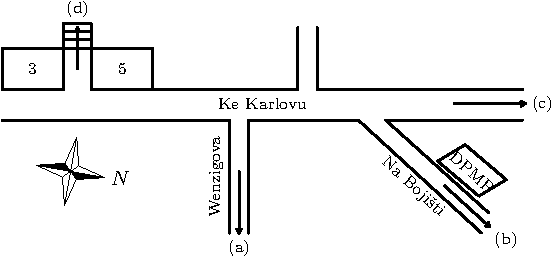
\includegraphics[width=0.7\textwidth]{karlov.pdf}\end{center}

\noindent{\it Vysvětlivky:\/} 3, 5: budovy Ke~Karlovu~3 (resp.~5),
(a): směr menza Budeč, (b): směr I.$\,$P.$\,$Pavlova (metro),
(c): směr Štěpánská (tramvaj), (d): směr menza Albertov,
DPMP: hlavní stan Dopravních podniků města Prahy.

\subsubsection{SCUK v~Hostivaři}
\begin{center}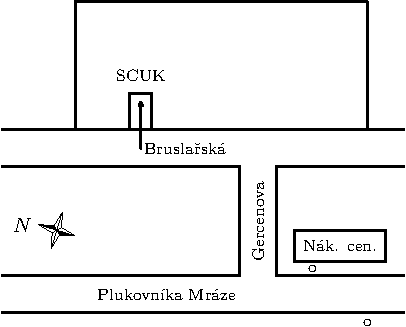
\includegraphics{hostivar.pdf}\end{center}

\noindent {\it Vysvětlivky:\/} SCUK: Sportovní centrum~UK, o: zastávka autobusu, Nák.~cen.: nákupní centrum.
\section{Závěr}

Tak a to je vše. Pokud jste dočetli až sem, věříme, že se vám
Kuchařka líbila, a že Vám informace v~ní obsažené byly k~užitku.
Pokud si myslíte, že v~ní něco není, a nebo naopak v~ní je něco,
co tam být nemá, ozvěte se na adresu \url{spolek@matfyzak.cz}.

\medskip

Přejeme Vám příjemné studium a hezký pobyt v~Praze.

\hskip 8cm \it Spolek Matfyzák
\newpage
\newpage
\pagenumbering{gobble}
\section*{Užitečné odkazy}
Máte v ruce mobilní telefon? Podívejte se na některé zajímavé odkazy hned!


\begin{tabular}{cc}
    
\includegraphics[width=4cm]{Images/QR/is.png}&
    
\includegraphics[width=4cm]{Images/QR/studijni.png} \\
    Studijní informační systém UK&
    Studijní oddělení MFF UK \\
    
    
\includegraphics[width=4cm]{Images/QR/skas.png}&
    
\includegraphics[width=4cm]{Images/QR/matfyzak.png} \\
    Studentská komora AS MFF UK &
    Spolek Matfyzák \\

    
\includegraphics[width=4cm]{Images/QR/facebook.png}&
    
\includegraphics[width=4cm]{Images/QR/knihovna.png} \\
    Skupina prváků na Facebooku &
    Knihovna MFF UK
\end{tabular}
		
	  
\end{document}